\documentclass[10pt, final]{IEEEtran}
%\documentclass[12pt, final, onecolumn]{IEEEtran}
%\documentclass[journal, final]{IEEEtran}
%
%allows for using the 1in margins on a page
%\usepackage{fullpage}
%allows for using graphics in the paper
\usepackage{graphicx}
%package needed to set the document into
%double space mode
\usepackage{setspace}
%allows for the use of subfigures
\usepackage{subfigure}
\usepackage{times}
\usepackage[table]{xcolor}
\usepackage{amsthm}
\usepackage{amsmath}
\usepackage{graphicx}
\usepackage{epstopdf}
\usepackage{algpseudocode}
\usepackage{algorithm}
\usepackage{caption}
\usepackage{float}
\usepackage{varwidth}
\usepackage{cite}
\usepackage[final]{pdfpages}
%\usepackage{algorithmic}
%\algsetup{linenosize=\small}
%\usepackage{latex8}
%
%% Define own float style called "algorithm"
%\makeatletter
%\newcommand\fs@algorithm{%
%  \let\@fs@capt\floatc@algorithm
%  \def\@fs@pre{\hrule height.8pt depth0pt\relax}% \kern2pt removed
%  \def\@fs@mid{\hrule\kern2pt}%  \kern2pt removed
%  \def\@fs@post{\kern2pt\hrule\relax}%
%  \let\@fs@iftopcapt\iftrue}
%\makeatother
%
%% Make the algorithm environment use the algorithm float style
%\floatstyle{algorithm}
%\restylefloat{algorithm}
\setlength{\floatsep}{10pt plus 2pt minus 2pt}
\setlength{\textfloatsep}{10pt plus 2pt minus 2pt}
\setlength{\intextsep}{10pt plus 2pt minus 2pt}

% Theorem Styles
\newtheorem{theorem}{Theorem}
\newtheorem{lemma}[theorem]{Lemma}
\newtheorem{proposition}[theorem]{Proposition}
\newtheorem{corollary}[theorem]{Corollary}
% Definition Styles
\theoremstyle{definition}
\newtheorem{definition}{Definition}
\newtheorem{example}{Example}
\theoremstyle{remark}
\newtheorem{remark}{Remark}

\newlength\myindent
\setlength\myindent{2em}
\newcommand\bindent{%
  \begingroup
  \setlength{\itemindent}{\myindent}
  \addtolength{\algorithmicindent}{\myindent}
}
\newcommand\eindent{\endgroup}

\captionsetup[table]{font=small,skip=0pt}
\captionsetup[figure]{font=small,skip=0pt}

%\textwidth 6.0in
%\textheight 8.5in

\textwidth 7in
\textheight 9in

\pagestyle{empty}

%Insert the title of the paper here
\title{Minimizing Cache Overhead via \\Loaded Cache Blocks and Preemption Placement}
%\title{Optimal Preemption Point Placement \\Using Interdependent Cache Related Preemption Delay}

%authors of the paper
\author{{John Cavicchio, Corey Tessler, and Nathan Fisher}
%Affiliation
\vspace{1.6mm}\\
\fontsize{10}{10}\selectfont\itshape
Wayne State University\\
\fontsize{9}{9}\selectfont\ttfamily\upshape
\{ba6444, corey.tessler, fishern\}@wayne.edu\\}

%in order to remove the date
\date{}

%begin document
\begin{document}


%title
\maketitle
%\pagestyle{plain}
\pagestyle{empty}

\thispagestyle{empty}
\begin{abstract}\label{sec:abstract}
Schedulability analysis for real-time systems has been the subject of prominent research over the past several decades.  One of the key foundations of schedulability analysis is an accurate worst case execution time (WCET) measurement for each task.  In real-time systems that support preemption, the cache related preemption delay (CRPD) can represent a significant component (up to 44\% as documented in research literature) \cite{pellizzoni:07,pellizzoni:08,pellizzoni:11} of variability to overall task WCET.  Several methods have been employed to calculate CRPD with significant levels of pessimism that may result in a task set erroneously declared as non-schedulable. Furthermore, they do not take into account that CRPD cost is inherently a function of where preemptions actually occur.  Our approach for computing CRPD via \emph{loaded cache blocks} (LCBs) is more accurate in the sense that cache state reflects which cache blocks and the specific program locations where they are reloaded.

Limited preemption models attempt to minimize preemption overhead (CRPD) by reducing the number of allowed preemptions and/or allowing preemption at program locations where the CRPD effect is minimized.  These algorithms rely heavily on accurate CRPD measurements or estimation models in order to identify an optimal set of preemption points.  Our approach improves the effectiveness of limited optimal preemption point placement algorithms by calculating the LCBs for each pair of adjacent preemptions to more accurately model task WCET and maximize schedulability as compared to existing preemption point placement approaches.  We propose an optimal preemption point placement algorithm using dynamic programming.  Lastly, we will demonstrate using a case study improved task set schedulability and optimal preemption point placement via our new LCB characterization.
%and synthetically generated task sets,
\end{abstract} 
\paragraph{Keywords:}
\label{sec:keywords}

Job scheduling, storage-aware scheduling, data-aware scheduling, 
data management, storage management, high-performance computing, 
scientific computing, data-intensive applications, SWAP


%\paragraph{Technical Area:}
\label{sec:tech_area}


Data Management
\section{Introduction}\label{sec:introduction}

%introduction
Hard-real-time systems differ from traditional computing systems in that one or more tasks must complete execution within a specified deadline, otherwise the utility of the result is severely diminished or utterly useless.  Ensuring hard-real-time task systems meet their corresponding deadlines is the subject of prominent research on schedulability analysis.  Paramount to schedulability analysis is accurate characterization of worst case execution time (WCET).  While the debate continues on whether non-preemptive versus fully preemptive execution is more effective, recent research on limited preemption models has shown to outperform non-preemptive and fully preemptive scheduling approaches in terms of the number of preemptions and schedulability when preemption cost is considered.  Non-preemptive execution has the disadvantage of introducing blocking of high priority tasks by lower priority tasks whereas fully preemptive execution has the disadvantage of subjecting preemption overhead which has shown to be up to 44\%~\cite{pellizzoni:07}~\cite{pellizzoni:08}~\cite{pellizzoni:11} of a tasks worst case execution time (WCET).  One of the prominent contributors to preemption overhead is due to cache related preemption delay (CRPD).  CRPD occurs when a task denoted \begin{math}\tau_{i}\end{math} is preempted by one or more higher priority tasks denoted \begin{math}\tau_{k}\end{math} whose execution results in the eviction of cache memory blocks that must be subsequently reloaded when task \begin{math}\tau_{i}\end{math} resumes execution.  Limited preemption approaches have the advantage of reduced blocking with a limited number of allowed preemptions while having the advantage of sections of non-preemptive regions (NPRs) reducing the preemption overhead.  One promising approach to implementing a limited preemption approach is selecting preemption points for each task subject to the constraint on maximum non-preemptive region execution time \begin{math}Q_{i}\end{math}.  A recent paper by Bertogna et. al.~\cite{bertogna:11} proposed and realized a polynomial time algorithm for selecting optimal preemption points for a linear basic block structure.  A linear basic block structure implies that conditional logic and branches are fully contained within basic block boundaries. CRPD literature permits basic blocks connected by arbitrary control flow graph structures.  The figure shown below illustrates the problem scope for selecting optimal preemption points for a linear basic block structure.

%outline of paper
The rest of this paper is organized as follows. First, current research efforts and related work in the areas of cache related preemption delay (CRPD) and limited preemption scheduling is discussed in Section~\ref{sec:related}.  Section~\ref{sec:system_model} describes the real-time task model terminology used in this paper.  The enhanced CRPD computation approach is detailed in Section~\ref{sec:crpd_computation}. Section~\ref{sec:schedulability_analysis} briefly outlines the impact of the revised CRPD computation approach incorporated into fixed priority (FP) and earliest deadline first (EDF) schedulability analysis.  The enhanced limited preemption point placement algorithm leverages the improved CPRD computation in a polynomial time algorithm as discussed in Section~\ref{sec:implementation}.  Synthetic task schedulability comparison of various preemption models in addition to a case study using well known bench mark tasks are presented and summarized in Section~\ref{sec:evaluation}.  Finally we will offer relevant conclusions along with proposed future work in Section~\ref{sec:conclusion}. 
%\vspace{-10pt}
\section{Related Work}\label{sec:related}

This paper draws from two areas of real-time theory resulting in two significant contributions. Hence, the descriptions of the related works are divided into two separate subsections, namely, CRPD Calculation, and Limited Preemption Scheduling.
\subsection {CRPD Calculation}\label{sec:crpd_related_work}
Analyzing the preempted task, Lee et al.~\cite{lee:96,lee:97,lee:98} introduced the concept and algorithm for computing the set of useful cache blocks (UCB) for statically addressed instruction and data for direct mapped and set-associative caches.
%where dynamic memory accesses are treated as cache misses.
The UCBs of the preempted task are used to compute an upper bound on the CRPD.
\newline
\indent
Analyzing the preempting task, Tomiyamay and Dutt~\cite{tomiyamay:00} computed the set of evicting cache blocks (ECBs) via program path analysis formulating an integer linear programming model for direct mapped instruction caches.
%The set of UCBs and ECBs can be computed using control flow graph (CFG) analysis of reaching memory blocks %(RMB) and live memory blocks %(LMB)~\cite{lee:96},~\cite{lee:97},~\cite{lee:98}.
In a similar fashion, the ECBs of the preempting task are used to compute the CRPD.
%which is again the cardinality of the ECB set times the cache block reload time (BRT).
Formal definitions of UCBs and ECBs were outlined by Altmeyer and Burguiere~\cite{altmeyer:11c}.  The preempting task’s memory accesses quantified as the set of evicting cache blocks will evict useful cache blocks thereby imposing non-negligible CRPD on the preempted task.

Complementary work by Negi et al.~\cite{negi:03} and Tan and Mooney~\cite{tan:04} compute the intersection of the ECB and UCB sets to achieve tighter bounds on the CRPD computation for direct-mapped and set-associative instruction caches.
%Negi`s work computes the set of UCBs and ECBs using the notion of reaching cache state and live cache state. This representation of the cache content enhances Lee`s original approach at the cost of higher computational complexity.
Staschulat and Ernst~\cite{staschulat:05c} realized an improvement in computational complexity at the expense of CRPD accuracy or tightness via a cache state reduction technique for direct mapped instruction caches that was later extended to address set-associative caches.
%This is accomplished by limiting the cache state size and selecting a revised cache state between two sets that %minimizes the set difference.
%One of the limitations with the existing UCB based analysis methods is their representation of memory blocks %that may reside in cache memory.  This over-approximation was employed to realize a safe bounds on CRPD which %is referred to as “may cache”~\cite{altmeyer:11c}.

Likewise, WCET analysis tools use an over-approximation to estimate cache misses and an under-approximation to estimate cache hits.  Cache hits are memory blocks that must reside in cache memory hence the term used to describe this set is “must cache”~\cite{altmeyer:11c}.  Altmeyer and Burguiere~\cite{altmeyer:11c} addressed this issue by introducing the notion of definitely-cached useful cache block (DC-UCB)~\cite{altmeyer:11c}.  The DC-UCB is useful in schedulability analysis to avoid double counting of cache misses resulting from intra-task cache block eviction.

Ramaprasad and Mueller~\cite{ramaprasad:06} examine the problem of dynamic addressing supporting CRPD analysis. Their algorithm employs memory access patterns to compute CRPD, instead of UCBs.  An important distinction to note is that instruction memory accesses are tightly coupled to the control flow graph in contrast to data memory accesses. This isomorphic property means the set of UCBs corresponding to data memory accesses changes more frequently thereby mandating UCB computation at the instruction level.
\subsection {Limited Preemption Scheduling}\label{sec:lp_related_work}
The motivation for limited preemption scheduling approaches stems from limitations of fully preemptive and non-preemptive scheduling.  Fully preemptive scheduling suffers from schedulability degradation due to increased preemption overhead penalties of which CRPD comprises a significant portion.  Non-preemptive scheduling suffers from reduced system utilization due to the blocking imposed on high priority jobs.  These factors have motivated research on alternative limited preemption scheduling approaches with the goal of achieving higher task utilization and reduced preemption overhead.

One such approach is known as the deferred preemption model.  The idea behind the deferred preemption model is to permit a currently executing job to execute non-preemptively for some period of time after the arrival of a high priority job.  Two distinct models of deferred preemption have been proposed by Burns~\cite{burns:05} and Baruah~\cite{baruah:05} known as the fixed preemption point model and the floating preemption point model respectively.

In the floating preemption point model~\cite{baruah:05}, the beginning of non-preemptive regions occur with the arrival of a higher priority job.  The currently executing job continues executing non-preemptively for \begin{math}Q_{i}\end{math} time units or earlier if the job completes execution. The location of the non-preemptive regions is nondeterministic or essentially floating. Baruah`s approach~\cite{baruah:05} computes the maximum amount of blocking time denoted \begin{math}Q_{i}\end{math} for which a task \begin{math}\tau_{i}\end{math} may execute non-preemptively while still preserving scheduling feasibility.

Another limited preemption scheduling technique known as preemption threshold scheduling was proposed by Wang and Saksena~\cite{wang:99}.  In preemption threshold scheduling, each task is assigned two priority values, namely, a nominal static priority \begin{math}p_{i}\end{math} and a preemption threshold \begin{math}\Pi_{i}\end{math}.  A task will be preempted only if the preempting task has a nominal priority \begin{math}p_{k}\end{math} greater than the preemption threshold \begin{math}\Pi_{i}\end{math}. In the fixed preemption point model~\cite{burns:05}, a task can be preempted only at a limited set of pre-defined locations. Basically, tasks contain a series of non-preemptive regions.  Preemptions are permitted at non-preemptive region boundaries or fixed preemption points.
\newline
\indent
Two closely related subsequent works implementing a fixed preemption point model for a fixed priority (FP) scheduler were proposed by Simonson and Patel~\cite{simonson:95} and by Lee et. al.~\cite{lee:98} whose objective was to reduce preemption overhead.  In Simonson’s and Patel’s approach~\cite{simonson:95}, tasks are sub-divided into distinct non-overlapping intervals, each constrained by the maximum blocking time \begin{math}Q_{i}\end{math} that higher priority tasks may be subjected to while preserving task set schedulability.  At a location within each interval containing the minimum number of UCBs, a single preemption point is placed.  Lee et. al.~\cite{lee:98} adopted a different method whereby the locations of preemption points are commensurate with the cardinality of the UCB set less than a pre-determined threshold.   While both techniques serve to improve preemption overhead over the fully preemptive approach, their heuristic nature is unable to achieve a globally optimal solution.  Complementary work by Bril et. al.~\cite{bril:14} recently integrated CRPD costs into fixed priority preemption threshold schedulability analysis for task sets with arbitrary deadlines.  Optimal priority thresholds are assigned via a CRPD cost minimization algorithm.
\newline
\indent
In contrast, Bertogna et. al.~\cite{bertogna:10} achieved an optimal preemption point placement algorithm with linear time complexity.  The analysis assumed a pessimistic fixed constant context switch cost at each preemption point equal to the largest preemption overhead experienced by a task.  Later work by Bertogna et. al.~\cite{bertogna:11} relaxes the fixed constant context switch assumption using more accurate variable preemption overhead cost information via available timing analysis tools.  Additionally, Peng et. al.~\cite{peng:14} proposed a pseudo-polynomial preemption point placement algorithm for control flow graphs with arbitrarily nested conditional program structures.  The CRPD cost model used in these papers does not take into account the interdependency between selected preemption points.
\newline
\indent
Our work improves these results by computing the cache related preemption delay (CRPD) contribution to the variable preemption overhead cost as a function of the current and next selected preemption points.  Our method not only accounts for the cache blocks evicted due to preemption, but also accounts for the cache blocks that are reloaded during execution between preemption points thereby improving the accuracy of marginal CRPD computations for multiple nested preemptions.
%Future work will incorporate our enhanced CRPD cost model into control flow graphs with arbitrarily nested %conditional program structures.
Due to the variability in CRPD and preemption overhead cost, we propose a dynamic programming algorithm to realize a globally optimal preemption point placement that further minimizes the number of preemptions and the preemption overhead cost due to the increased CRPD accuracy.
%The dynamic programming algorithm assumes a linear basic block structure with high level programming language %constructs fully contained within the basic block.

%\section{Bibliography}\label{sec:bibliography}

\subsection {Paper References}\label{sec:paper_references}
~\cite{altmeyer:11} ~\cite{hanninen:11} ~\cite{yao:10} ~\cite{altmeyer:12} ~\cite{altmeyer:11b} ~\cite{marinho:12} ~\cite{bastoni:11} ~\cite{marinho:11} ~\cite{buttazzo:13} ~\cite{negi:03} ~\cite{staschulat:05} ~\cite{tomiyamay:00} ~\cite{staschulat:04} ~\cite{altmeyer:09} ~\cite{ju:07} ~\cite{ramaprasad:06} ~\cite{bertogna:10} ~\cite{sebek:01}  ~\cite{bertogna:11}  ~\cite{staschulat:05b}  ~\cite{staschulat:05c}  ~\cite{zhang:07} ~\cite{ramaprasad:08} ~\cite{schliecker:10} ~\cite{ramaprasad:10}  ~\cite{staschulat:04b}  ~\cite{lv:10}  ~\cite{chakraborty:09} ~\cite{kleinsorge:11}  ~\cite{ramaprasad:09}  ~\cite{schliecker:10b} ~\cite{mezzetti:10} ~\cite{lunniss:13} ~\cite{davis:06} ~\cite{zhang:12} ~\cite{lunniss:12} ~\cite{altmeyer:10b}  ~\cite{chattopadhyay:13}  ~\cite{puaut:09} ~\cite{peng:13}  ~\cite{prete:09} ~\cite{marinho:12b} ~\cite{davis:12} ~\cite{lee:96} ~\cite{tan:04}  ~\cite{lee:98}  ~\cite{lee:97} ~\cite{bastoni:10}  ~\cite{davis:13} ~\cite{petters:01} ~\cite{lee:01} ~\cite{ramaprasad:06b} ~\cite{busquets-mataix:96} ~\cite{hardy:09} ~\cite{dobrin:04} ~\cite{yao:10b} ~\cite{altmeyer:09b}   ~\cite{davis:13b} ~\cite{vera:03} ~\cite{bertogna:11b} ~\cite{marinho:12c} ~\cite{bertogna:11c}  ~\cite{yao:11} ~\cite{marinho:13} ~\cite{marinho:12d} ~\cite{yao:09} ~\cite{buttazzo:13} ~\cite{wilhelm:08}  ~\cite{baldovin:13} ~\cite{davis:13c} ~\cite{schneider:00} ~\cite{staschulat:06} ~\cite{puaut:06} ~\cite{chakraborty:11} ~\cite{burns:05} ~\cite{baruah:05} ~\cite{wang:99} ~\cite{simonson:95}  ~\cite{altmeyer:11c} ~\cite{pellizzoni:07} ~\cite{pellizzoni:08} ~\cite{pellizzoni:11} ~\cite{tessler:14}
\section{System Model}\label{sec:system_model}

Our system contains a task set \begin{math}\tau\end{math} of $n$ periodic or sporadic tasks (\begin{math}\tau_{1}\end{math}, \begin{math}\tau_{2}\end{math}, ..., \begin{math}\tau_{j}\end{math}, ..., \begin{math}\tau_{n}\end{math}) each scheduled on a single processor.  Each task \begin{math}\tau_{i}\end{math} is characterized by a tuple (\begin{math}\phi_{i}\end{math}, \begin{math}C_{i}^{NP}\end{math}, \begin{math}D_{i}\end{math}, \begin{math}T_{i}\end{math}, \begin{math}J_{i}\end{math}, \begin{math}P_{i}\end{math}) where \begin{math}\phi_{i}\end{math} is the starting time (also known as the phase), \begin{math}C_{i}^{NP}\end{math} is the non-preemptive worst case execution time, \begin{math}D_{i}\end{math} is the relative deadline, \begin{math}T_{i}\end{math} is the inter-arrival time or period, \begin{math}J_{i}\end{math} is the release jitter and \begin{math}P_{i}\end{math} is the uniquely assigned static fixed priority.  Each task \begin{math}\tau_{i}\end{math} creates an infinite number of jobs, with the first job arriving at starting time \begin{math}\phi_{i}\end{math} and subsequent jobs arriving no earlier than \begin{math}T_{i}\end{math} time units with a relative deadline \begin{math}D_{i}\end{math} \begin{math}\leq\end{math} \begin{math}T_{i}\end{math}.  The system utilizes a preemptive scheduler with each task/job containing \begin{math}N_{i}\end{math} number of basic blocks denoted (\begin{math}\delta_{i,1}\end{math}, \begin{math}\delta_{i,2}\end{math}, ..., \begin{math}\delta_{i,N_{i}}\end{math}) with the total number of basic blocks given by N = \begin{math}\Sigma_{i}\end{math} \begin{math}N_{i}\end{math}. In existing literature, basic blocks are denoted as \begin{math}\delta_{i,j}\end{math} where $i$ is the task identifier and $j$ is the basic block identifier denoting the basic block position in the control flow graph.  We introduce the notation \begin{math}\delta_{j}^{i}\end{math} where $i$ is the task identifier and $j$ is the basic block identifier. A basic block is a set of one or more instructions that execute non-preemptively.  Basic blocks are essentially the vertices $V$ of a control flow graph (CFG) connected by edges $E$ representing the execution sequence of job instructions. Preemptions are permitted at basic block boundaries.  Non-preemptive (NP) basic block execution time denoted as \begin{math}b_{i,j}\end{math} where $i$ is the task identifier and $j$ is the basic block identifier, where
\begin{equation}\label{eqn:c-np1}
    C_{i}^{NP} = \Sigma_{j}\ b_{i,j}.
\end{equation}
\noindent
We introduce the notation \begin{math}b_{j}^{i}\end{math} where $i$ is the task identifier and $j$ is the basic block identifier, hence using this convention we have
\begin{equation}\label{eqn:c-np2}
    C_{i}^{NP} = \Sigma_{j}\ b_{j}^{i}.
\end{equation}
\noindent
The task release jitter \begin{math}J_{i}\end{math} is defined as the maximum time between the task arriving for execution and it being released to a state of being ready to execute.  In our work, we assume the release jitter \begin{math}J_{i}\end{math} = 0.  The processor utilization \begin{math}U_{i}\end{math} of task \begin{math}\tau_{i}\end{math} is given by
\begin{equation}\label{eqn:u-task}
    U_{i} = C_{i}^{NP}/T_{i}.
\end{equation}
\noindent
Blocking time \begin{math}B_{i}\end{math} is the time which task \begin{math}\tau_{i}\end{math} is subject to accounting for the maximum time that a lower priority task either executes non-preemptively or holds a resource that is shared with task \begin{math}\tau_{i}\end{math} or any other task of equal or higher priority.

%In our work, we remove the restriction of a linear basic block structure thereby permitting an arbitrarily %connected basic block structure.  
A direct-mapped cache is assumed, though the techniques described here can be readily extended to set- associative caches. Tasks may be preempted by multiple higher-priority tasks identified by the variable $k$ where
\begin{equation}\label{eqn:hp-tasks}
    k \in hp(i) = \{k | P_{k} > P_{i}\}.
\end{equation}
\noindent
comprising the set of higher priority tasks for task \begin{math}\tau_{i}\end{math}.  This set needs to be filtered by tasks that must preempt during the execution window of task \begin{math}\tau_{i}\end{math}.  The number of times task \begin{math}\tau_{k}\end{math} can preempt task \begin{math}\tau_{i}\end{math} during task \begin{math}\tau_{i}\end{math}'s execution is given by the term
\begin{equation}\label{eqn:num-preemptions}
    N_{p}(\tau_{i},\tau_{k})=\lceil(C_{i}^{NP} + J_{k})/T_{k})\rceil \geq 1.
\end{equation}
\noindent
where $k$ is the index of the preempting task \begin{math}\tau_{k}\end{math} and $i$ is the index of the preempted task \begin{math}\tau_{i}\end{math}.  In a limited preemption approach, each task is permitted to execute non-preemptively for a maximum amount of time denoted by \begin{math}Q_{i}\end{math}.  The following figure shown below illustrates the linear basic block connection structure \begin{math}\delta_{i,b}\end{math} also denoted as \begin{math}\delta_{b}^{i}\end{math} using our convention.


%\vspace{-5pt}
\section{CRPD Computation}\label{sec:crpd_computation}

While existing research has focused on computing the upper bounds on cache related preemption delay (CRPD), our approach achieves higher accuracy by computing the \emph{loaded cache blocks} (LCBs) due to higher priority task preemption by using the set of potential/chosen preemption locations.  Consistent with the literature the sets of various cache blocks are represented as sets of integers.  We employ the CRPD terms UCB and ECB as defined by Lee et. al.~\cite{lee:98} and by Altmeyer and Burguiere~\cite{altmeyer:11c}.
%Since the variables P and Q in the original are overloaded here, we modify the definition alternatively using %basic block identifiers.

\begin{definition}
\textbf{Useful Cache Block (UCB)}: A memory block $m$ is called a useful cache block at program point \begin{math}\delta_{i}^{j_{1}}\end{math}, if \\(a) $m$ may be cached at \begin{math}\delta_{i}^{j_{1}}\end{math} and \\(b) $m$ may be reused at program point \begin{math}\delta_{i}^{j_{2}}\end{math} that may be reached from \begin{math}\delta_{i}^{j_{1}}\end{math} without eviction of $m$ on this path.
\end{definition}

%\Leftrightarrow
\noindent More formally, cache-set \begin{math}s \in \textit{UCB}(\tau_{i})\textrm{ if and only if }\tau_{i}\end{math} has a useful cache block in cache-set $s$.  Note this definition of \textit{UCB} embodies a task level view.  Cache-set \begin{math}s \in \textit{UCB}_{\textrm{out}}(\delta_{i}^{j})\textrm{ if and only if }\delta_{i}^{j}\end{math} has a useful cache block in cache-set $s$ where
\begin{equation}\label{eqn:ucb-task}
    \textit{UCB}(\tau_{i}) = \bigcup_{\delta_{i}^{j} \in \tau_{i}} \textit{UCB}_{\textrm{out}}(\delta_{i}^{j}).
\end{equation}
\noindent The notation \begin{math}\textit{UCB}_{\textrm{out}}(\delta_{i}^{j})\end{math} is the set of useful cache blocks cached in task \begin{math}\tau_{i}\end{math} post execution of basic block \begin{math}\delta_{i}^{j}\end{math}.  Similarly, the notation \begin{math}\textit{UCB}_{in}(\delta_{i}^{j})\end{math} is the set of useful cache blocks cached in task \begin{math}\tau_{i}\end{math} pre-execution of basic block \begin{math}\delta_{i}^{j}\end{math}.

\begin{definition}
\textbf{Evicting cache block (ECB)}: A memory block of the preempting task is called an evicting cache block, if it may be accessed during the execution of the preempting task.
\end{definition}

%\Leftrightarrow
\noindent Cache-set \begin{math}s \in \textit{ECB}(\tau_{k})\textrm{ if and only if }\tau_{k}\end{math} may evict a cache block in cache-set $s$.  Note this definition of \textit{ECB} also embodies a task level view.  Cache-set \begin{math}s \in \textit{ECB}(\delta_{i}^{j})\textrm{ if and only if } \delta_{k}^{j}\end{math} may evict a cache block in cache-set $s$ where
\begin{equation}\label{eqn:ecb-task}
    \textit{ECB}(\tau_{k}) = \bigcup_{\delta_{k}^{j} \in \tau_{k}} \textit{ECB}(\delta_{k}^{j}).
\end{equation}
\noindent The notation \begin{math}\textit{ECB}(\delta_{k}^{j})\end{math} is the set of evicting cache blocks accessed in task \begin{math}\tau_{k}\end{math} during execution of basic block \begin{math}\delta_{k}^{j}\end{math}.  In order to determine which cache blocks are reloaded once preemption occurs, we introduce the notion of an accessed useful cache block (AUCB).
%
%Altmeyer and Burguiere~\cite{altmeyer:11c} introduced a refinement of \textit{UCB} to capture extrinsic cache %blocks evicted due to inter-task preemption thereby removing the cache blocks evicted via intra-task %execution.
%
%\begin{definition}
%\textbf{Definitely Cached Useful Cache Block (DC-UCB)}: A memory block $m$ is called a definitely cached useful %cache block at program point \begin{math}\delta_{i}^{j_{1}}\end{math}, if \\(a) $m$ must be cached at %\begin{math}\delta_{i}^{j_{1}}\end{math} and \\(b) $m$ may be reused at program point %\begin{math}\delta_{i}^{j_{2}}\end{math} that may be reached from \begin{math}\delta_{i}^{j_{1}}\end{math} %without eviction of $m$ on this path.
%\end{definition}
%
%\noindent More formally, cache-set \begin{math}s \in \textit{DC-UCB}(\tau_{i}) if and only if %\tau_{i}\end{math} has a definitely cached useful cache block in cache-set $s$.  Note this definition of %\textit{DC-UCB} also embodies a task level view.  Cache-set \begin{math}s \in %\textit{DC-UCB}_{\textrm{out}}(\delta_{i}^{j})\textit{ if and only if }\delta_{i}^{j}\end{math} has a definitely cached useful %cache block in cache-set $s$ where
%
%\begin{equation}\label{eqn:dcucb-task}
%    \textit{DC-UCB}(\tau_{i}) = \bigcup_{j} \textit{DC-UCB}_{\textrm{out}}(\delta_{i}^{j}).
%\end{equation}
%
%\noindent The notation
%\begin{math}\textit{DC-UCB}_{\textrm{out}}(\delta_{i}^{j})\end{math} is the set of definitely cached useful cache blocks %cached in task \begin{math}\tau_{i}\end{math} post execution of basic block %\begin{math}\delta_{i}^{j}\end{math}.  Similarly, the notation %\begin{math}\textit{DC-UCB}_{in}(\delta_{i}^{j})\end{math} is the set of definitely cached useful cache blocks %cached in task \begin{math}\tau_{i}\end{math} pre-execution of basic block %\begin{math}\delta_{i}^{j}\end{math}.

%To capture the notion of what we are attempting to count, consider the set of replaced cache blocks (RCBs).
%
%\begin{definition}
%\textbf{Replaced cache block (RCB)}: A memory block of the preempted task is called a replaced cache block, if %it is replaced during the execution of a preempting task.
%\end{definition}
%
%\noindent \begin{math}\textit{RCB}_{\textrm{out}}(\delta_{i}^{j},\tau_{k})\end{math} denotes preemption of task %\begin{math}\tau_{i}\end{math} by task \begin{math}\tau_{k}\end{math} occurring immediately after basic block %\begin{math}\delta_{i}^{j}\end{math}, where task \begin{math}\tau_{i}\end{math} at basic block location %\begin{math}\delta_{i}^{j}\end{math} is a potential/selected preemption point in our preemption point placement %algorithm described later.  We compute the set of replaced cache blocks (RCBs) as follows:
%\begin{equation}\label{eqn:rcb-formula}
%    \textit{RCB}_{\textrm{out}}(\delta_{i}^{j},\tau_{k}) = \textit{DC-UCB}_{\textrm{out}}(\delta_{i}^{j}) \cap
%    \textit{ECB}(\tau_{k}).
%    \textit{RCB}_{\textrm{out}}(\delta_{i}^{j},\tau_{k}) = \textit{UCB}_{\textrm{out}}(\delta_{i}^{j}) \cap %\textit{ECB}(\tau_{k}).
%\end{equation}
%
%\noindent where \begin{math}\textit{DC-UCB}_{\textrm{out}}(\delta_{i}^{j})\end{math} is the set of definitely cached %useful cache blocks for task \begin{math}\tau_{i}\end{math} post basic block
%\noindent where \begin{math}\textit{UCB}_{\textrm{out}}(\delta_{i}^{j})\end{math} is the set of useful cache blocks for %task \begin{math}\tau_{i}\end{math} post basic block \begin{math}\delta_{i}^{j}\end{math} execution; and %\begin{math}\textit{ECB}(\tau_{k})\end{math} is the set of extrinsic evicting cache blocks of the preempting %task \begin{math}\tau_{k}\end{math}.
%\noindent
%If a cache block is evicted there are two options in terms of where the preemption overhead cost can be paid: %1) the cost can be paid where the next memory accesses occur; or 2) The cost can also be paid where the %preemptions occur.  In order to determine which cache blocks are reloaded once preemption occurs, we introduce %the notion of an accessed useful cache block (AUCB).
%If a cache block is evicted the cost is paid where the preemptions occur.

\begin{definition}
\textbf{Accessed useful cache block (AUCB)}: A memory block of the preempted task is called an accessed useful cache block; if it may be accessed during the execution of a basic block \begin{math}\delta_{i}^{j}\end{math} for task \begin{math}\tau_{i}\end{math}.
\end{definition}

%\noindent The term \begin{math}\textit{AUCB}_{\textrm{out}}(\delta_{i}^{j})\end{math} represents the definitely cached %useful cache blocks (DC-UCBs) accessed by task \begin{math}\tau_{i}\end{math} at during execution of basic %block
\noindent The term \begin{math}\textit{AUCB}_{\textrm{out}}(\delta_{i}^{j})\end{math} represents the useful cache blocks (UCBs) accessed by task \begin{math}\tau_{i}\end{math} at during execution of basic block at location \begin{math}\delta_{i}^{j}\end{math}. The definition of \textit{AUCB} is introduced to capture the set of task accessed memory at a specific basic block location subsequently used in the calculation of blocks that must be reloaded when task preemptions occur.  We compute the set of accessed useful cache blocks (AUCBs) as follows:
\begin{equation}\label{eqn:aucb-formula}
%    \textit{AUCB}_{\textrm{out}}(\delta_{i}^{j}) = \textit{DC-UCB}_{\textrm{out}}(\delta_{i}^{j}) \cap
%    \textit{ECB}(\delta_{i}^{j}).
    \textit{AUCB}_{\textrm{out}}(\delta_{i}^{j}) = \textit{UCB}_{\textrm{out}}(\delta_{i}^{j}) \cap \textit{ECB}(\delta_{i}^{j}).
\end{equation}
%\noindent where \begin{math}\textit{DC-UCB}_{\textrm{out}}(\delta_{i}^{j})\end{math} is the set of definitely cached %useful cache blocks for task \begin{math}\tau_{i}\end{math} post basic block
\noindent where \begin{math}\textit{UCB}_{\textrm{out}}(\delta_{i}^{j})\end{math} is the set of useful cache blocks for task \begin{math}\tau_{i}\end{math} post basic block \begin{math}\delta_{i}^{j}\end{math} execution; and \begin{math}\textit{ECB}(\delta_{i}^{j})\end{math} denotes the set of cache blocks accessed in task \begin{math}\tau_{i}\end{math} during execution of basic block \begin{math}\delta_{i}^{j}\end{math}. It is important to note that only cache block evictions due to preemption are considered, as intrinsic cache misses are captured as part of WCET analysis in the term \begin{math}C_{i}^{NP}\end{math}.  Using the previously defined terms, we may now define and explicitly compute the cache blocks that are re-loaded due to preemption which are called loaded cache blocks (LCBs).

\begin{definition}
\textbf{Loaded cache block (LCB)}: A memory block of the preempted task is called a loaded cache block, if it may be re-loaded during the execution following a preempting task.
\end{definition}
\noindent
\begin{math}\textit{LCB}(\delta_{i}^{curr},\delta_{i}^{next})\end{math} denotes set set of cache blocks re-loaded during execution of the non-preemptive region between basic block \begin{math}\delta_{i}^{curr}\end{math} and basic block \begin{math}\delta_{i}^{next}\end{math}, resulting from preemption of task \begin{math}\tau_{i}\end{math}, where basic block location \begin{math}\delta_{i}^{curr}\end{math} and \begin{math}\delta_{i}^{next}\end{math} are the potential/selected preemption point and next potential/selected preemption point respectively.

The definition of \textit{LCB} is introduced to capture the set of reloaded cache memory at a specific basic block as a function of the current and next selected preemption points.  Here, we account for the overhead within a non-preemptive region (i.e., series of basic blocks with no preemptions) for reloading UCBs that could have potentially been evicted by the preemption occurring immediately after $\delta_i^{curr}$ and used by some basic block prior to the preemption occurring immediately after $\delta_i^{next}$.
%As previously stated, there are two options in terms of where the cache block reload cost can be paid: 1) the cost can be paid where the next memory %accesses occur; or 2) The cost can also be paid where the preemptions occur.  In this paper, we use the cost paid where the preemptions occur as per %below.
%This results in two similar formulations for computing loaded cache blocks (LCBs) as per below.
%\newline
%\newline
%\noindent\textbf{Preemption Cost Paid Where Preemptions Occur}
\begin{equation}\label{eqn:lcb-formula-1}
\begin{split}
%    \lefteqn{\textit{LCB}(\delta_{i}^{curr},\delta_{i}^{next},\tau_{k}) =} & \\
%    &\left[\textit{DC-UCB}_{\textrm{out}}(\delta_{i}^{curr})\ \cap \left[\cup_\lambda
%    \textit{AUCB}_{\textrm{out}}(\delta_{i}^{\lambda})\right]\right] \cap \textit{ECB}(\tau_{k})\\
    \lefteqn{\textit{LCB}(\delta_{i}^{curr},\delta_{i}^{next}) =} & \\
    &\left[\textit{UCB}_{\textrm{out}}(\delta_{i}^{curr})\ \cap \left[\cup_{\nu \in \lambda} \textit{AUCB}_{\textrm{out}}(\delta_{i}^{\nu})\right]\right] \cap [\cup_{\tau_{k}\in hp_(i)} \textit{ECB}(\tau_{k})]\\
\end{split}
\end{equation}

%\newline
\noindent
where
\begin{equation*}\label{eqn:lcb-formula-1b}
    \lambda \stackrel{\text{def}}{=} \{ \nu|\nu \in [ \textit{curr}, \textit{curr}+1, \ldots, \textit{next} ] \}
\end{equation*}

\noindent
%\begin{math}\textit{AUCB}_{\textrm{out}}(\delta_{i}^{x})\end{math} represents the accessed useful cache blocks or memory of interest accessed by the preempted %task \begin{math}\tau_{i}\end{math} at basic block \begin{math}\delta_{i}^{x}\end{math};
\begin{math}\delta_{i}^{curr}\end{math} represents the current selected preemption point where \begin{math}\delta_{i}^{curr} \in \rho(\tau_{i})\end{math} and \begin{math}\delta_{i}^{next}\end{math} represents the next selected preemption point where \begin{math}\delta_{i}^{next} \in \rho(\tau_{i})\end{math}.  This formula for \begin{math}\textit{LCB}(\delta_{i}^{curr},\delta_{i}^{next})\end{math} results in the accounting of loaded cache blocks where the preemption occurs.  Note that this notation assumes a sequential basic block structure. Once we have the set of cache blocks that must be re-loaded due to preemption, the CRPD related preemption overhead may be computed as shown below.
%\newline
%\newline
%\noindent\textbf{Preemption Cost Paid Where Memory Reloads Occur}
%\begin{equation}\label{eqn:lcb-formula-2}
%\begin{split}
%    \lefteqn{\textit{LCB}(\delta_{i}^{j},\tau_{k}) =} & \\
%    &\left[\cup_\varphi \left[\textit{RCB}_{\textrm{out}}(\delta_{i}^{\varphi},\tau_{k}) \setminus \cup_\lambda
%    \textit{AUCB}_{\textrm{out}}(\delta_{i}^{\lambda})\right] \cap \textit{AUCB}_{\textrm{out}}(\delta_{i}^{j})\right]\\
%\end{split}
%\end{equation}
%\noindent
%where
%\begin{equation*}\label{eqn:lcb-formula-2b}
%\varphi \stackrel{\text{def}}{=} \{\kappa | (\kappa \geq \delta_{i}^{1} \wedge \kappa < \delta_{i}^{j})\}
%\end{equation*}
%\begin{equation*}\label{eqn:lcb-formula-2c}
%    \lambda \stackrel{\text{def}}{=} \{\nu | (\nu > \delta_{i}^{\varphi} \wedge \nu \leq
%     min(\delta_{i}^{j},\rho_{next}(\delta_{i}^{\varphi})))\}
%\end{equation*}
%
%\noindent
%Using the term \begin{math}\textit{LCB}(\delta_{i}^{j},\tau_{k})\end{math}, we can compute the preemption cost %as a function of the current and next selected preemption point:
%\begin{equation}\label{eqn:lcb-formula-3}
%\textit{LCB}(\delta_{i}^{curr},\delta_{i}^{next},\tau_{k}) = [\cup_\lambda %\textit{LCB}(\delta_{i}^{\lambda},\tau_{k})]
%\end{equation}
%
%\newline
%\noindent
%where
%\begin{equation*}\label{eqn:lcb-formula-1b}
%    \lambda \stackrel{\text{def}}{=} \{ \nu|\nu \in [ \delta_{i}^{curr} \text{,} \delta_{i}^{next} ] \}
%\end{equation*}
%
%\noindent
%\begin{math}\textit{AUCB}_{\textrm{out}}(\delta_{i}^{x})\end{math} represents the accessed useful cache blocks or memory %of interest accessed by the preempted task \begin{math}\tau_{i}\end{math} at basic block %\begin{math}\delta_{i}^{x}\end{math}; and \begin{math}\delta_{i}^{j}\end{math} represents the current basic %block location.  This formula for \begin{math}\textit{LCB}(\delta_{i}^{j},\tau_{k})\end{math} results in the %accounting of loaded cache blocks where the reload occurs.  The algorithms for optimal preemption placement for %linear basic block structure use the preemption cost paid where The preemptions occur formula.
%Once we have the set of cache blocks that must be re-loaded due to preemption, the CRPD related preemption %overhead may be computed as per below.
\begin{equation}\label{eqn:crpd-formula}
    \gamma_{i}(\delta_{i}^{curr},\delta_{i}^{next}) = | \textit{LCB}(\delta_{i}^{curr},\delta_{i}^{next}) | \cdot BRT.
\end{equation}

\noindent where BRT is the cache block reload time; and \begin{math}\textit{LCB}(\delta_{i}^{curr},\delta_{i}^{next})\end{math} represents the loaded cache blocks or memory accessed by the preempted task \begin{math}\tau_{i}\end{math} at basic block \begin{math}\delta_{i}^{curr}\end{math} caused by higher priority preempting tasks.
%\newline
%\newline
%\noindent
%To illustrate our approach for performing CRPD computations, consider the following example as shown below.
%\vspace{-10pt}

\vspace{-5pt}
\section{Integrated WCET/CRPD Calculation}\label{sec:schedulability_analysis}

The modified preemption cost as a function of the current and next preemption points is given by:
\begin{equation}\label{eqn:prempt-cost}
\begin{split}
    \xi_{i}(\delta_{i}^{curr},\delta_{i}^{next})\ =\ &\gamma_{i}(\delta_{i}^{curr},\delta_{i}^{next}) + \pi + \sigma + \\ &\eta(\gamma_{i}(\delta_{i}^{curr},\delta_{i}^{next})).
\end{split}
\end{equation}
%
\noindent
where \begin{math}\pi\end{math} is the pipeline cost, \begin{math}\sigma\end{math} is the scheduler processing cost, and \begin{math}\eta()\end{math} is the front side bus contention resulting from the cache reload interference as described in~\cite{pellizzoni:07,pellizzoni:08,pellizzoni:11}.
%Commensurate with our worst case analysis, the preemption overhead cost as a function of the current and next %selected preemption points is:
%\begin{equation}\label{eqn:prempt-cost}
%    \xi_{i}(\delta_{i}^{curr},\delta_{i}^{next}) = \textit{max}_{k \in hp(i)} [ %\xi_{i}(\delta_{i}^{curr},\delta_{i}^{next},\tau_{k})].
%\end{equation}
%
The output of our algorithm is an optimal set of preemption points, with respect to our computed preemption cost $\xi_i()$, subject to the maximum allowable non-preemption region \begin{math}Q_{i}\end{math}.  The optimal set of preemption points obtained using the enhanced accuracy of our preemption cost computation is used to calculate each task's WCET with preemption overhead given by:
\vspace{-5pt}
\begin{equation}\label{eqn:wcet-cost}
   C_{i} = B_{i}(\rho_{i}) = C_{i}^{NP} + \sum_{m=1}^{|\rho_{i}|-1} [\xi_{i}(\rho_{i}^{m},\rho_{i}^{m+1})]
\end{equation}
\noindent
%where $\rho_i \subseteq \{\delta_i^0, \delta_i^1,  \ldots, \delta_i^{N_i}\}$ is an ordered set by ascending %index of selected preemption points for task \begin{math}\tau_{i}\end{math}:
%%\begin{math}\rho_{i}\end{math} is the set of selected preemption points for task
%\begin{equation*}\label{eqn:pp-set}
%\begin{split}
%   \rho_{i} \stackrel{\text{def}}{=} \{\delta_{i}^{m}|&\delta_{i}^{m} \text{ is a selected preemption point of %task } \tau_{i}\ \\ &\wedge m \in [0, %1, 2, \ldots, N_{i}]\}
%\end{split}
%\end{equation*}
%%
%\noindent
where \begin{math}\rho_{i}^{m}\end{math} is the \textrm{$m^{th}$} selected preemption point for task \begin{math}\tau_{i}\end{math}.  To further clarify what we mean by preemption, we say that $\delta_i^m$ is a ``preemption point'' if the preemption between basic blocks $\delta_i^m$ and $\delta_i^{m+1}$ is enabled, meaning the scheduler may preempt between these two basic blocks.  Commensurate with our preemption point placement algorithm discussed later, preemptions are always taken at basic blocks $\delta_i^0$ and $\delta_i^{N_i}$ hence $\delta_i^0,\ \delta_i^{N_i}\ \in\ \rho_{i}$ for any feasible set of preemption points $\rho_i$.  Supplemental clarification of this requirement is shown in the example of LCB interdependence in the appendix.
%\begin{equation*}\label{eqn:pp-mth}
%\begin{split}
%   \rho_{i}^{m} \stackrel{\text{def}}{=} \{\delta_{i}^{j}|&\delta_{i}^{j} \text{ is the $m^{th}$ selected %preemption point of task } \tau_{i}\ \\ &\wedge j \in [0, 1, 2, \ldots, N_{i}]\}
%\end{split}
%\end{equation*}
%
\noindent
The complete problem formulation with constraints for finding the minimum WCET with preemption overhead cost \begin{math}B_{i}(\rho_{i})\end{math} for task \begin{math}\tau_{i}\end{math} is given by:
\begin{equation}\label{eqn:global-bbkwcet-cost}
\begin{split}
   B_{i}(\rho_{i}) = \min_{\rho_{i} \in \tau_{i}} \Big\{&\Big[\sum_{m=1}^{|\rho_{i}|-1} \xi_{i}(\rho_{i}^{m},\rho_{i}^{m+1}) + \sum_{s=1}^{N_i}b_{i}^{s}\Big]\ |\\
   &\Psi_{i}(\rho_{i})\ =\ True\Big\}
\end{split}
\end{equation}
%
\noindent
The selection of optimal preemption points is subject to the constraint \begin{math}\Psi_{i}(\rho_{i})\end{math} that no non-preemptive region in task \begin{math}\tau_{i}\end{math} exceeds the maximum allowable non-preemption region parameter \begin{math}Q_{i}\end{math}:
\begin{equation}\label{eqn:global-pp-constraint}
   \Psi_{i}(\rho_{i}) =
\left\{
\begin{array}{lr}
    \textrm{True, }&\textrm{if } q_{i}^{m}(\rho_{i}) \leq Q_{i} \textrm{ for } m \in [1,|\rho_{i}|-1] \\
    \textrm{False, }&\textrm{otherwise}
\end{array}
\right\}~
\end{equation}
%
\noindent
where \begin{math}q_{i}^{m}(\rho_{i})\end{math} represents the \begin{math}m^{th}\end{math} non-preemptive-region (NPR) time for task \begin{math}\tau_{i}\end{math}, capturing the cost of the preemption $\rho_i^m$ given that $\rho_i^{m+1}$ is the next selected preemption point, plus the basic block cost of all blocks between $\rho_i^m$ and $\rho_i^{m+1}$:
\begin{equation}\label{eqn:global-mthnpr-time}
   q_{i}^{m}(\rho_{i}) = \Big[\xi_{i}(\rho_{i}^{m},\rho_{i}^{m+1}) +
   \sum_{s: \delta_i^s \in \{\rho_i^m,\ldots, \rho_i^{m+1}\}} b_{i}^{s}\Big]
\end{equation}
\noindent
%\newline
Our approach employs the results of schedulability analysis and the aforementioned WCET + CRPD calculation with the maximum allowable non-preemption region parameter \begin{math}Q_{i}\end{math} computed for each task \begin{math}\tau_{i}\end{math}.  The objective is to select a subset of preemption points that minimizes each tasks WCET + CRPD parameter \begin{math}C_{i}\end{math}. We introduce slight variations of terms \begin{math}\Psi_{i}\end{math}, \begin{math}q_{i}\end{math}, and \begin{math}B_{i}\end{math}, used in solving intermediate sub-problems of our proposed algorithm.  The selection of optimal preemption points is subject to the constraint that no non-preemptive region in task \begin{math}\tau_{i}\end{math} exceeds the maximum allowable non-preemption region parameter \begin{math}Q_{i}\end{math}:
\begin{equation}\label{eqn:pp-constraint}
   \Psi_{i}(\delta_{i}^{j},\delta_{i}^{k}) =
\left\{
\begin{array}{lr}
    \textrm{True, }&\textrm{if } q_{i}(\delta_{i}^{j},\delta_{i}^{k}) \leq Q_{i} \textrm{ for } \delta_{i}^{j},\delta_{i}^{k} \in \rho_{i} \\
    \textrm{False, }&\textrm{otherwise}
\end{array}
\right\}~
\end{equation}
\noindent
where \begin{math}q_{i}(\delta_{i}^{j},\delta_{i}^{k})\end{math} represents a possible candidate optimal non-preemptive-region (NPR) time with successive preemption points at basic block locations \begin{math}\delta_{i}^{j}\end{math} and \begin{math}\delta_{i}^{k}\end{math} for task \begin{math}\tau_{i}\end{math}:
\begin{equation}\label{eqn:mthnpr-time}
   q_{i}(\delta_{i}^{j},\delta_{i}^{k}) = \Big[\xi_{i}(\delta_{i}^{j},\delta_{i}^{k}) + \sum_{n=j+1}^{k}b_{i}^{n}\Big]
\end{equation}
\noindent
The next expression gives a recursive solution to the CRPD+WCET minimization problem for the subproblem of the first $i$ basic blocks.  We compute the WCET including the preemption point $\delta_i^k$ using the term \begin{math}B_{i}(\delta_{i}^{k})\end{math} for task \begin{math}\tau_{i}\end{math} as given by:
%We propose an O(N!) recursive relation shown in equation (\ref{eqn:bbkwcet-cost}) that computes the WCET %including preemption cost used in the dynamic programming algorithm for selecting the optimal preemption %points. While the recursive formulation is clearly inefficient, it is helpful in developing an understanding of %how the algorithm works. We compute the WCET including preemption cost for each potential preemption point %\begin{math}\delta_{i}^{k}\end{math} using the term \begin{math}B_{i}(\delta_{i}^{k})\end{math} for task %\begin{math}\tau_{i}\end{math} as given by:
%\begin{equation}\label{eqn:bbkwcet-cost-old}
%\begin{split}
%   B_{i}(\delta_{i}^{k}) = \min_{m \in \{0,1, \ldots, k-1\}}
%   \Big\{\Big[&B_{i}(\delta_{i}^{m}) + q_{i}(\delta_{i}^{m},\delta_{i}^{k})\Big]\ |\\
%   &\Psi_{i}(\delta_{i}^{m},\delta_{i}^{k})\ =\ True\Big\}
%\end{split}
%\end{equation}
%
\begin{equation}\label{eqn:bbkwcet-cost}
\begin{split}
   B_{i}(\delta_{i}^{k}) = \min_{m \in \{0,1, \ldots, k-1\}}
   \Big\{\Big[&B_{i}(\delta_{i}^{m}) + q_{i}(\delta_{i}^{m},\delta_{i}^{k})\Big]\ |\\
   &\Psi_{i}(\delta_{i}^{m},\delta_{i}^{k})\ =\ True\Big\}
%\wedge\\&k\ \in\ \{1, 2, \ldots, N_i\}\Big\}
\end{split}
\end{equation}
%\newline
\noindent
when $k\ \in\ \{1, 2, \ldots, N_i\}$.  For the base case where $\textrm{k = 0}$, we have $B_{i}(\delta_{i}^{0}) = 0$.  This recursive formulation is necessary for developing the dynamic programming solution presented in the next section.  The following theorem shows our problem has optimal substructure, and thus the formulation of Equation~\ref{eqn:bbkwcet-cost} represents an optimal solution.
%In accordance with the recursive nature of equation (\ref{eqn:bbkwcet-cost}) we propose an O(N!) recursive %algorithm shown in Algorithm~\ref{alg:recursive-optimal-ppp} for computing the optimal preemption points.  %While the recursive formulation is clearly inefficient, it is helpful in developing an understanding of how the %algorithm works.
%\noindent
%\begin{equation}\label{eqn:global-pp-constraint}
%   \Psi_{i}(\rho_{i}) =
%\left\{
%\begin{array}{lr}
%    \textrm{True, }&\textrm{if } q_{i}^{m}(\rho_{i}) \leq Q_{i} \textrm{ for } m \in [1,|\rho_{i}|-1] \\
%    \textrm{False, }&\textrm{otherwise}
%\end{array}
%\right\}~
%\end{equation}
%
%\noindent
%where \begin{math}q_{i}^{m}(\rho_{i})\end{math} represents the \begin{math}m^{th}\end{math} %non-preemptive-region (NPR) time for task \begin{math}\tau_{i}\end{math}:
%\begin{equation}\label{eqn:global-mthnpr-time}
%   q_{i}^{m}(\rho_{i}) = \Big[\xi_{i}(\rho_{i}^{m},\rho_{i}^{m+1}) + %\sum_{n=\rho_{i}^{m}}^{\rho_{i}^{m+1}}b_{i}^{n}\Big]
%\end{equation}
%
%\noindent
%In accordance with the recursive nature of equation (\ref{eqn:bbkwcet-cost}) we propose an O(N!) recursive %algorithm shown in Algorithm~\ref{alg:recursive-optimal-ppp} for computing the optimal preemption points.  %While the recursive formulation is clearly inefficient, it is helpful in developing an understanding of how the %algorithm works.  Starting with the first basic block and for each successive basic block %\begin{math}\delta_{i}^{m}, m \in [1,N_{i}]\end{math}, the overall WCET cost is computed for two cases: 1) %\begin{math}\delta_{i}^{m} \in \rho_{i}\end{math}, and 2) \begin{math}\delta_{i}^{m} \not\in %\rho_{i}\end{math}.  At each step of the algorithm the set \begin{math}\rho_{i}\end{math} must conform to the %constraint of equation (\ref{eqn:pp-constraint}).  Once basic block \begin{math}\delta_{i}^{N_{i}}\end{math} %has been examined, the set of selected preemption points is given by \begin{math}\rho_{i} = %\rho_{i}^{(N_{i})}\end{math}.  The WCET cost with basic block \begin{math}\delta_{i}^{m}\end{math} included in %the set of potential preemption points is given by:
%\begin{equation}\label{eqn:pcost-bb}
%p_{COST}(\delta_{i}^{m})\ =\ B_{i}^{0,m}(\rho_{i}) + B_{i}^{m,N_{i}}(\rho_{i})
%\end{equation}
%
%The WCET cost with basic block \begin{math}\delta_{i}^{m}\end{math} excluded from the set of potential %preemption points is given by:
%\begin{equation}\label{eqn:npcost-bb}
%n_{COST}(\delta_{i}^{m})\ =\ B_{i}^{0,m-1}(\rho_{i}) + b_{i}^{m} + B_{i}^{m+1,N_{i}}(\rho_{i})
%\end{equation}
%%
%\noindent
%where \begin{math}B_{i}^{k,m}\end{math} is the WCET with preemption overhead of basic blocks $k$ to $m$ of task %\begin{math}\tau_{i}\end{math} as given by:
%\begin{equation}\label{eqn:global-bbkwcet-cost}
%\begin{split}
%   B_{i}^{k,m}(\rho_{i}) = \min_{\delta_{i}^{j} \in \tau_{i}} \Big[&B_{i}^{j-1}(\rho_{i}(\delta_{i}^{j-1})) + %\\ &\xi_{i}(\delta_{i}^{j},\rho_{i}^{next}(\delta_{i}^{j})) + \sum_{n=k}^{m}b_{i}^{n}\Big]
%\end{split}
%\end{equation}
%%
%\noindent
%where the term \begin{math}\rho_{i}^{next}(\delta_{i}^{j})\end{math} is the next potential/selected preemption %point from basic block \begin{math}\delta_{i}^{j}\end{math}:
%\begin{equation}\label{eqn:ppnext-set}
%\begin{split}
%   \rho_{i}^{next}(\delta_{i}^{k}) \stackrel{\text{def}}{=} \{\delta_{i}^{j}|&\delta_{i}^{k} = \rho_{i}^{m} %\wedge \delta_{i}^{j} = \rho_{i}^{m+1} \\ &\textrm{ for some } m \in [1,N_{i}-1]\}
%\end{split}
%\end{equation}
%{\fontsize{10}{10}\selectfont
%\begin{algorithm}
%\caption{Recursive Optimal Preemption Point Placement}
%\label{alg:recursive-optimal-ppp}
%\begin{algorithmic}[0]
%\small
%\State \textbf{\underline{Step 0:}}
%%\\
%\State {$\ \ \rho_{i}^{(0)}\ \gets\ \{\delta_{i}^{0},\delta_{i}^{N_{i}}\}$};
%\State {$\ \ \textbf{if}\ \Psi_{i}^{N_{i}}(\{\delta_{i}^{0},\delta_{i}^{1},\delta_{i}^{2}, ..., %\delta_{i}^{N_{i}}\}) = False$\ \textbf{then}}
%\State {$\ \ \ \ \ \ \textbf{return}\ \textbf{INFEASIBLE;}$}
%\State {$\ \ \textbf{end if}$}
%\\
%\State \textbf{\underline{Step 1:}}
%\begin{equation*}
%\rho^{(1)}\ \gets\
%\left\{
%\begin{array}{l}
%    \rho^{(0)}, if\ n_{COST}(\delta_{i}^{1}) < p_{COST}(\delta_{i}^{1})\ \&\ \ \ \ \ \ \ \ \ \ \ \\
%    \ \ \ \ \ \ \ \ \ \ \Psi_{i}^{1}(\rho^{(0)}) = True\\
%    \rho^{(0)}\ \cup\ \delta_{i}^{1},\ otherwise
%\end{array}
%\right\}~
%\end{equation*}
%\State \textbf{\underline{Step 2:}}
%\begin{equation*}
%\rho^{(2)}\ \gets\
%\left\{
%\begin{array}{l}
%    \rho^{(1)}, if\ n_{COST}(\delta_{i}^{2}) < p_{COST}(\delta_{i}^{2})\ \&\ \ \ \ \ \ \ \ \ \ \ \\
%    \ \ \ \ \ \ \ \ \ \ \Psi_{i}^{2}(\rho^{(1)}) = True\\
%    \rho^{(1)}\ \cup\ \delta_{i}^{2},\ otherwise
%\end{array}
%\right\}~
%\end{equation*}
%\ldots
%\State \textbf{\underline{Steps m = 1,\ \ldots,\ $N_{i}$:}}
%\begin{equation*}
%\rho_{i}^{(m)}\ \gets\
%\left\{
%\begin{array}{l}
%    \rho_{i}^{(m-1)}, if\ n_{COST}(\delta_{i}^{m}) < p_{COST}(\delta_{i}^{m})\ \&\ \ \ \ \\
%    \ \ \ \ \ \ \ \ \ \ \ \ \ \Psi_{i}^{m}(\rho_{i}^{(m-1)}) = True\\
%    \rho_{i}^{(m-1)}\ \cup\ \delta_{i}^{m},\ otherwise
%\end{array}
%\right\}~
%\end{equation*}
%\ldots
%\State \textbf{\underline{Step $N_{i}$:}}
%\begin{equation*}
%\rho^{(N_{i})}\ \gets\
%\left\{
%\begin{array}{l}
%    \rho^{(N_{i}-1)}, if\ n_{COST}(\delta_{i}^{N_{i}}) < p_{COST}(\delta_{i}^{N_{i}})\ \&\\
%    \ \ \ \ \ \ \ \ \ \ \ \ \ \ \Psi_{i}^{N_{i}}(\rho^{(N_{i}-1)}) = True\\
%    \rho^{(N_{i}-1)}\ \cup\ \delta_{i}^{N_{i}},\ otherwise
%\end{array}
%\right\}~
%\end{equation*}
%\normalsize
%\end{algorithmic}
%\end{algorithm}
%}
%
\begin{theorem}
\label{thm:optimal-substructure-cost}
The WCET + CRPD cost variable $B_{i}(\delta_{i}^{k})$ utilized in Equation~\ref{eqn:bbkwcet-cost} exhibits optimal substructure.
\end{theorem}
%
%\noindent
%We now prove the optimal substructure property of the WCET + CRPD cost $B_{i}(\delta_{i}^{j},\delta_{i}^{k})$.
%\newline
\noindent
\begin{proof}
%Let $B_{i}(\delta_{i}^{k})$ with its corresponding selected preemption points denoted by $\rho_{i}^{k}$ be the optimal limited preemption execution cost solution from basic block $\delta_{i}^{0}$ to basic block $\delta_{i}^{k}$, and assume the optimal cost solution contains the basic block identified by $\delta_{i}^{m}$. Furthermore, let $B_{i}(\delta_{i}^{m})$ with selected preemption points denoted by $\rho_{i}^{m}$ and $q_{i}(\delta_{i}^{m},\delta_{i}^{k})$ be the optimal limited preemption execution cost from $\delta_{i}^{0}$ to $\delta_{i}^{m}$, respectively, contained in the optimal solution to the original problem. Three additional constraints are imposed where $\rho_{i}^{m} \subseteq \rho_{i}^{k}$ with $B_{i}(\delta_{i}^{m}) + q_{i}(\delta_{i}^{m},\delta_{i}^{k}) = B_{i}(\delta_{i}^{k})$.
Let $\Delta_i^k$ be the subproblem of the sequential control flowgraph containing basic blocks $\{\delta_i^0, \delta_i^1, \ldots, \delta_i^{k}\}$.
To prove optimal substructure, we show that we can obtain the optimal set of preemption points for minimizing the WCET+CRPD for any $\Delta_i^k$ by using the optimal solutions to subproblems $\Delta_i^0, \Delta_i^1, \ldots, \Delta_i^{k-1}$.  Let $B_i(\delta_i^0), B_i(\delta_i^1), \ldots, B_i(\delta_i^{k-1})$ represent the cost of the optimal solution to these subproblems.  We need to show that Equation~\ref{eqn:bbkwcet-cost} represents the optimal cost to $\Delta_i^k$.

By way of contradiction, assume there is a better feasible solution $\rho_{i}'$ for the sub-problem of determining the optimal limited preemption execution costs from basic block $\delta_{i}^{0}$ to basic block $\delta_{i}^{k}$; that is, $B_{i}(\rho_{i}')$ is strictly smaller than the solution to $\Delta_i^k$ obtained in Equation~\ref{eqn:bbkwcet-cost} (i.e.,  $B_{i}(\delta_{i}^{k})$).  Let $\delta_i^{\ell}$ (where $\ell \in \{0, 1, \ldots, k-1\}$) be the last preemption point prior to $\delta_i^k$ in the set $\rho_{i}'$, and let $\rho_{i}''$ be the set of preemption points obtained from $\rho_{i}'$ by removing the preemption point after $\delta_i^k$ (i.e., $\rho_{i}''$ is a solution to $\Delta_i^{\ell}$).  Thus, we can represent the cost of the solution $\rho_{i}'$ (i.e., $B_i(\rho_{i}')$ by the left-hand-side of the following inequality:
\begin{equation}\label{eqn:bi-deltai-lb}
    B_i(\rho_{i}'') + q_i(\delta_i^{\ell}, \delta_i^k) < B_i(\delta_i^k).
\end{equation}

Since $\rho_{i}'$ is a feasible solution to $\Delta_i^k$, it must be that $\Psi_i(\delta_i^{\ell}, \delta_i^k)$ is true.  Hence, from Equation~\ref{eqn:bbkwcet-cost} and the $\min$ operation, we can obtain an upper bound on $B_i(\delta_i^k)$ by considering the solution to subproblem $\Delta_i^{\ell}$:
\begin{equation}\label{eqn:bi-deltai-ub}
    B_i(\delta_i^k) \leq B_i(\delta_i^{\ell}) + q_i(\delta_i^{\ell}, \delta_i^k).
\end{equation}

Combining the inequalities of Equations~\ref{eqn:bi-deltai-lb} and~\ref{eqn:bi-deltai-ub}, we finally obtain $B_i(\rho_{i}'') < B_i(\delta_i^{\ell})$.  However, this contradicts our assumption at the beginning of the proof that $B_i(\delta_i^{\ell})$ represented an optimal solution to subproblem $\Delta_i^{\ell}$.  Thus, a solution $\rho_{i}'$ with smaller cost than $B_i(\delta_i^k)$ cannot exist, and Equation~\ref{eqn:bbkwcet-cost} computes the minimum obtainable cost for the problem $\Delta_i^k$.
%Since the solution for selecting the optimal preemption points from basic block $\delta_{i}^{0}$ to basic block $\delta_{i}^{k}$ will work regardless of which set of preemption points are used, we could then use the better solution  $B_{i}^{'}(\delta_{i}^{m})$ and $\rho_{i}^{'m}$ to arrive at a lower cost solution to the original problem. Thus we have the following:
%\begin{equation}\label{eqn:pcost-bb-1}
%B_{i}(\delta_{i}^{k})\ =\ B_{i}(\delta_{i}^{m}) + q_{i}(\delta_{i}^{m},\delta_{i}^{k})
%\end{equation}
%\begin{equation}\label{eqn:pcost-bb-2}
%B_{i}(\delta_{i}^{k})\ >\ B_{i}^{'}(\delta_{i}^{m}) + q_{i}^{'}(\delta_{i}^{m},\delta_{i}^{k})
%\end{equation}
%\noindent
%However this contradicts the original definition that $B_{i}(\delta_{i}^{k})$ and $\rho_{i}^{k}$ form an optimal solution to the problem. Therefore, the optimal limited preemption execution cost from basic block $\delta_{i}^{0}$ to basic block $\delta_{i}^{k}$ contained in the original solution $B_{i}(\delta_{i}^{k})$ and $\rho_{i}^{k}$ must be an optimal solution to the sub-problem of determining the optimal limited preemption execution cost solution from basic block $\delta_{i}^{0}$ to basic block $\delta_{i}^{k}$. Thus, the problem exhibits optimal substructure.
\end{proof}

\vspace{-10pt}
\section{Preemption Point Placement Algorithm}\label{sec:implementation}

Our approach employs the results of schedulability analysis and the aforementioned WCET + CRPD calculation with the maximum allowable non-preemption region parameter \begin{math}Q_{i}\end{math} computed for each task \begin{math}\tau_{i}\end{math}.  The objective is to select a subset of preemption points that minimizes each tasks WCET + CRPD parameter \begin{math}C_{i}\end{math}. The selection of optimal preemption points is subject to the constraint that no non-preemptive region in task \begin{math}\tau_{i}\end{math} exceeds the maximum allowable non-preemption region parameter \begin{math}Q_{i}\end{math}:
\begin{equation}\label{eqn:pp-constraint}
   \Psi_{i}(\rho_{i}) =
\left\{
\begin{array}{lr}
    \textrm{True, }&\textrm{if } q_{i}^{m}(\rho_{i}) \leq Q_{i} \textrm{ for } m \in [1,|\rho_{i}|-1] \\
    \textrm{False, }&\textrm{otherwise}
\end{array}
\right\}~
\end{equation}

\noindent
where \begin{math}q_{i}^{m}(\rho_{i})\end{math} represents the \begin{math}m^{th}\end{math} non-preemptive-region (NPR) time for task \begin{math}\tau_{i}\end{math}:
\begin{equation}\label{eqn:mthnpr-time}
   q_{i}^{m}(\rho_{i}) = \Big[\xi_{i}(\rho_{i}^{m},\rho_{i}^{m+1}) + \sum_{n=\rho_{i}^{m}}^{\rho_{i}^{m+1}}b_{i}^{n}\Big]
\end{equation}

\noindent
In accordance with the recursive nature of equation (\ref{eqn:bbkwcet-cost}) we propose an O(N!) recursive algorithm shown in Algorithm~\ref{alg:recursive-optimal-ppp} for computing the optimal preemption points.  While the recursive formulation is clearly inefficient, it is helpful in developing an understanding of how the algorithm works.  Starting with the first basic block and for each successive basic block \begin{math}\delta_{i}^{m}, m \in [1,N_{i}]\end{math}, the overall WCET cost is computed for two cases: 1) \begin{math}\delta_{i}^{m} \in \rho_{i}\end{math}, and 2) \begin{math}\delta_{i}^{m} \not\in \rho_{i}\end{math}.  At each step of the algorithm the set \begin{math}\rho_{i}\end{math} must conform to the constraint of equation (\ref{eqn:pp-constraint}).  Once basic block \begin{math}\delta_{i}^{N_{i}}\end{math} has been examined, the set of selected preemption points is given by \begin{math}\rho_{i} = \rho_{i}^{(N_{i})}\end{math}.  The WCET cost with basic block \begin{math}\delta_{i}^{m}\end{math} included in the set of potential preemption points is given by:
\begin{equation}\label{eqn:pcost-bb}
p_{COST}(\delta_{i}^{m})\ =\ B_{i}^{0,m}(\rho_{i}) + B_{i}^{m,N_{i}}(\rho_{i})
\end{equation}

The WCET cost with basic block \begin{math}\delta_{i}^{m}\end{math} excluded from the set of potential preemption points is given by:
\begin{equation}\label{eqn:npcost-bb}
n_{COST}(\delta_{i}^{m})\ =\ B_{i}^{0,m-1}(\rho_{i}) + b_{i}^{m} + B_{i}^{m+1,N_{i}}(\rho_{i})
\end{equation}

{\fontsize{10}{10}\selectfont
\begin{algorithm}
\caption{Recursive Optimal Preemption Point Placement}
\label{alg:recursive-optimal-ppp}
\begin{algorithmic}[0]
\small
\State \textbf{\underline{Step 0:}}
%\\
\State {$\ \ \rho_{i}^{(0)}\ \gets\ \{\delta_{i}^{0},\delta_{i}^{N_{i}}\}$};
\State {$\ \ \textbf{if}\ \Psi_{i}^{N_{i}}(\{\delta_{i}^{0},\delta_{i}^{1},\delta_{i}^{2}, ..., \delta_{i}^{N_{i}}\}) = False$\ \textbf{then}}
\State {$\ \ \ \ \ \ \textbf{return}\ \textbf{INFEASIBLE;}$}
\State {$\ \ \textbf{end if}$}
\\
%\State \textbf{\underline{Step 1:}}
%\begin{equation*}
%\rho^{(1)}\ \gets\
%\left\{
%\begin{array}{l}
%    \rho^{(0)}, if\ n_{COST}(\delta_{i}^{1}) < p_{COST}(\delta_{i}^{1})\ \&\ \ \ \ \ \ \ \ \ \ \ \\
%    \ \ \ \ \ \ \ \ \ \ \Psi_{i}^{1}(\rho^{(0)}) = True\\
%    \rho^{(0)}\ \cup\ \delta_{i}^{1},\ otherwise
%\end{array}
%\right\}~
%\end{equation*}
%\State \textbf{\underline{Step 2:}}
%\begin{equation*}
%\rho^{(2)}\ \gets\
%\left\{
%\begin{array}{l}
%    \rho^{(1)}, if\ n_{COST}(\delta_{i}^{2}) < p_{COST}(\delta_{i}^{2})\ \&\ \ \ \ \ \ \ \ \ \ \ \\
%    \ \ \ \ \ \ \ \ \ \ \Psi_{i}^{2}(\rho^{(1)}) = True\\
%    \rho^{(1)}\ \cup\ \delta_{i}^{2},\ otherwise
%\end{array}
%\right\}~
%\end{equation*}
%\ldots
\State \textbf{\underline{Steps m = 1,\ \ldots,\ $N_{i}$:}}
\begin{equation*}
\rho_{i}^{(m)}\ \gets\
\left\{
\begin{array}{l}
    \rho_{i}^{(m-1)}, if\ n_{COST}(\delta_{i}^{m}) < p_{COST}(\delta_{i}^{m})\ \&\ \ \ \ \\
    \ \ \ \ \ \ \ \ \ \ \ \ \ \Psi_{i}^{m}(\rho_{i}^{(m-1)}) = True\\
    \rho_{i}^{(m-1)}\ \cup\ \delta_{i}^{m},\ otherwise
\end{array}
\right\}~
\end{equation*}
%\ldots
%\State \textbf{\underline{Step $N_{i}$:}}
%\begin{equation*}
%\rho^{(N_{i})}\ \gets\
%\left\{
%\begin{array}{l}
%    \rho^{(N_{i}-1)}, if\ n_{COST}(\delta_{i}^{N_{i}}) < p_{COST}(\delta_{i}^{N_{i}})\ \&\\
%    \ \ \ \ \ \ \ \ \ \ \ \ \ \ \Psi_{i}^{N_{i}}(\rho^{(N_{i}-1)}) = True\\
%    \rho^{(N_{i}-1)}\ \cup\ \delta_{i}^{N_{i}},\ otherwise
%\end{array}
%\right\}~
%\end{equation*}
\normalsize
\end{algorithmic}
\end{algorithm}
}
\noindent
The recursive formulation gives a preliminary algorithm description, however, it is computationally intractable.  We now propose an \begin{math}O(cN^{2})\end{math} dynamic programming algorithm for computing the optimal preemption points.  In support of our dynamic programming algorithm, we propose the following theorem claiming optimal substructure of our solution formulation in terms of the WCET + CRPD cost $B_{i}$.

\begin{theorem}
\label{thm:optimal-substructure-cost}
The WCET + CRPD cost variable $B_{i}$ utilized in our solution exhibits optimal substructure.
\end{theorem}

\noindent
We now prove the optimal substructure property of the WCET + CRPD cost $B_{i}$.
\newline
\noindent
\begin{proof}
Let $B_{i}^{j,k}(\rho_{i})$ with its corresponding selected preemption points denoted by $\rho_{i}^{j,k}$ be the optimal limited preemption execution cost solution from basic block $j$ to basic block $k$, and assume the optimal cost solution contains the basic block identified by $m$. Furthermore, let $B_{i}^{j,m}(\rho_{i})$ with selected preemption points denoted by $\rho_{i}^{j,m}$ and $B_{i}^{m+1,k}(\rho_{i})$ with selected preemption points denoted by $\rho_{i}^{m+1,k}$ be the optimal limited preemption execution cost from $j$ to $m$ and from $m+1$ to $k$, respectively, contained in the optimal solution to the original problem. Three additional constraints are imposed where $\rho_{i}^{j,m} \subseteq \rho_{i}^{j,k}$ and $\rho_{i}^{m+1,k} \subseteq  \rho_{i}^{j,k}$ with $B_{i}^{j,m}(\rho_{i}) + B_{i}^{m+1,k}(\rho_{i}) = B_{i}^{j,k}(\rho_{i})$. To prove optimal substructure, we need to prove that in order for the limited preemption execution cost $B_{i}^{j,k}(\rho_{i})$ to be optimal, the limited preemption execution costs $B_{i}^{j,m}(\rho_{i})$ and $B_{i}^{m+1,k}(\rho_{i})$ must also be optimal solutions to their respective sub-problems.

Using proof by contradiction, assume there is a better solution $B_{i}^{'j,m}(\rho_{i}^{'})$ for the sub-problem of determining the optimal limited preemption execution costs from basic block j to basic block m, such that $B_{i}^{'j,m}(\rho_{i}^{'}) < B_{i}^{j,m}(\rho_{i})$ and $\rho_{i}^{'j,m} \neq \rho_{i}^{j,m}$. Since the solution for selecting the optimal preemption points from basic block j to k will work regardless of which set of preemption points are used between basic block j and basic block k, we could then use the better solution  $B_{i}^{'j,m}(\rho_{i}^{'})$ and $\rho_{i}^{'j,m}$ to arrive at a lower cost solution to the original problem. Thus we have the following:
\begin{equation}\label{eqn:pcost-bb-1}
B_{i}^{j,k}(\rho_{i})\ =\ B_{i}^{j,m}(\rho_{i}) + B_{i}^{m+1,k}(\rho_{i})
\end{equation}
\begin{equation}\label{eqn:pcost-bb-2}
B_{i}^{j,k}(\rho_{i})\ >\ B_{i}^{'j,m}(\rho_{i}^{'}) + B_{i}^{'m+1,k}(\rho_{i}^{'})
\end{equation}
\noindent
However this contradicts the original definition that $B_{i}^{j,k}(\rho_{i})$ and $\rho_{i}^{j,k}$ form an optimal solution to the problem. Therefore, the optimal limited preemption execution cost from basic block j to basic block k contained in the original solution $B_{i}^{j,k}(\rho_{i})$ must be an optimal solution to the sub-problem of determining the optimal limited preemption execution cost solution from basic block j to basic block k. The same argument works for the sub-problem of determining the optimal limited preemption execution cost solution from basic block m+1 to basic block k. Thus, the problem exhibits optimal substructure.
\end{proof}
\noindent
\newline
The algorithm is summarized in Algorithm~\ref{alg:dynamic-optimal-ppp} shown below.  For each task $\tau_i$, we are given the following parameters: 1) the number of basic blocks $N_i$ , 2) the non-preemptive execution time of each basic block $b_i$, 3) the maximum allowable non-preemptive region $Q_i$, and 4) the preemption cost matrix $\xi_i$.  The preemption cost matrix $\xi_i$ is organized for each basic block \begin{math}\delta_{i}^{j}\end{math} and contains the preemption cost for all successor basic blocks of the task's control flow graph.  The minimum (preemptive or non-preemptive) cost between all basic blocks is computed and stored in a matrix denoted $B_{i}$.  The $B_{i}$ matrix is initially seeded with the non-preemptive cost for basic block pairs that satisfy the constraint $q_{i}(\delta_{i}^{j},\delta_{i}^{k}) < Q_{i}$. All other entries are set to infinity.  As we consider whether each basic block $\delta_{i}^{k}$ is in the set of optimal preemption points, the location of the previous basic block $\delta_{i}^{j}$ with minimal preemption cost is stored in an array denoted $\rho_{prev}$.  The algorithm examines each basic block from \begin{math}\delta_{i}^{1}\end{math} to \begin{math}\delta_{i}^{N_i}\end{math} to minimize the preemption cost by traversing backwards from the current basic block $\delta_{i}^{k}$ under consideration in order to find the basic block $\delta_{i}^{j}$ with minimal preemption cost subject to the constraint $q_{i}(\delta_{i}^{j},\delta_{i}^{k}) < Q_{i}$.  While each basic block will have a predecessor with minimum preemption cost, the list of selected preemption points is obtained by starting with basic block $\delta_{i}^{N_i}$ and hopping to the predecessor basic block stored at $\rho_{prev}(\delta_{i}^{N_i})$, denoted $\delta_{i}^{m}$.  Basic blocks $\delta_{i}^{N_i}$ and $\delta_{i}^{m}$ are added to the optimal preemption point set $\rho_{i}$.  This basic block hopping process continues until basic block $\delta_{i}^{0}$ is reached.  The set $\rho_{i}$ contains the complete list of selected optimal preemption points.
{\fontsize{10}{10}\selectfont
\begin{algorithm}
\caption{D.P. Optimal Preemption Point Placement}
\label{alg:dynamic-optimal-ppp}
\begin{algorithmic}[1]
\small
\Function{$Select\_Optimal\_PPP$}{$N_{i}$,$b_{i}$,$Q_{i}$,$\xi_i$}
\State {$N_{p}\ \gets\ \infty\ q_{i}\ \gets\ \infty\ B_{i}\ \gets\ \infty\ \rho_{prev}\ \gets\ \{\delta_{i}^{0}\}$};
\If {$b_{i}^{k} > Q_{i}\ for\ some\ k\ \in\ [1,N_{i}]$}
\State\Return{INFEASIBLE;}
\EndIf
\For{$k: 2\leq k\leq N_{i}$}
\State\Call{$Compute\_PPCost$}{$\delta_{i}^{k-1}$,$\delta_{i}^{k}$};
\For{$j: k-1\geq j\geq 1\ and\ q_{i}(\delta_{i}^{j},\delta_{i}^{k}) < Q_{i}$}
%\Comment{$Check\ preemption\ cost\ at\ BB\ \delta_{i}^{j}\ with\ preemption$}
%\Comment{$at\ BB\ \delta_{i}^{0}\ and\ BB\ \delta_{i}^{k}$}
\State\Call{$Compute\_PPCost$}{$\delta_{i}^{0}$,$\delta_{i}^{j}$};
\State\Call{$Compute\_PPCost$}{$\delta_{i}^{j}$,$\delta_{i}^{k}$};
\State{$P_{cost}\ \gets\ B_{i}(\delta_{i}^{0},\delta_{i}^{j})\ +\ B_{i}(\delta_{i}^{j},\delta_{i}^{k})$};
\If {$P_{cost} < B_{i}(\delta_{i}^{0},\delta_{i}^{k})$}
\State{$B_{i}(\delta_{i}^{0},\delta_{i}^{k}) \gets P_{cost}$};
\State{$\rho_{prev}(\delta_{i}^{k}) \gets \delta_{i}^{j}$};
\EndIf
\EndFor
\EndFor
\State{$\rho_{i}\ \gets\ $\Call{$Compute\_PPSet$}{$N_{i},\rho_{prev}$}};
\State\Return{FEASIBLE;}
\EndFunction
\\
\Function{$Compute\_PPCost$}{$\delta_{i}^{j}$,$\delta_{i}^{k}$}
\If {$q_{i}(\delta_{i}^{j},\delta_{i}^{k})$ = $\infty$}
\State{$Compute\ \xi_{i}(\delta_{i}^{j}$,$\delta_{i}^{k})\ using\ Equation\ (\ref{eqn:prempt-cost})$};
\State{$Compute\ N_{p}(\delta_{i}^{j}$,$\delta_{i}^{k})$};
\State{$Compute\ q_{i}(\delta_{i}^{j}$,$\delta_{i}^{k})$};
\If {$q_{i}(\delta_{i}^{j}$,$\delta_{i}^{k})\ \leq\ Q_{i}$}
\State{$B_{i}(\delta_{i}^{j},\delta_{i}^{k}) \gets q_{i}(\delta_{i}^{j}$,$\delta_{i}^{k})$};
\State{$\rho_{prev}(\delta_{i}^{k}) \gets \delta_{i}^{j}$};
\Else
\If {$j-k\ =\ 1$}
\State\Return{INFEASIBLE;}
\EndIf
\EndIf
\EndIf
\EndFunction
\\
\Function{$Compute\_PPSet$}{$N_{i}$,$\rho_{prev}$}
\State {Computes $\rho_{i}$ from $\rho_{prev}$ (Details omitted)}
%\State {$\rho_{i}\ \gets\ \{\}$};
%\State {$\rho_{index}\ \gets\ \{\delta_{i}^{N_{i}}\}$};
%\While {$\rho_{index}\ \neq\ \delta_{i}^{0}$}
%\State {$\rho_{i}\ \gets\ \rho\ \cup \rho_{index}$};
%\State {$\rho_{index}\ \gets\ \rho_{prev}(\rho_{index})$};
%\EndWhile
%\State {$\rho_{i}\ \gets\ \rho_{i}\ \cup \rho_{index}$};
%\State\Return{$\rho_{i}$;}
\EndFunction
\normalsize
\end{algorithmic}
\end{algorithm}
}
%\showthe\floatsep 12pt
%\showthe\textfloatsep 20pt
%\showthe\intextsep 12pt
To exemplify how our algorithm works, consider the following example.
\begin{figure}[h!]
\vspace{-10pt}
\begin{center}
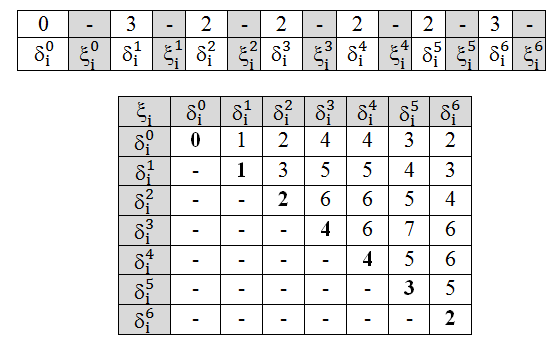
\includegraphics[width=0.45\textwidth]{algo_example.png}
\caption{Algorithm Example.}
\label{fig:algo_example}
\end{center}
\vspace{-10pt}
\end{figure}
Let $N_i=6$ and $Q_i=12$ for the following basic block structure with WCET and preemption costs shown in Figure~\ref{fig:algo_example}.  The algorithm computes and stores the cumulative non-preemptive execution costs for starting and ending basic block pairs in a matrix denoted $N_p$.  Using this information, the combined WCET and CRPD costs for each basic block pair is computed and stored in a matrix denoted $q_{i}$.  These matrices are shown in Figure~\ref{fig:algo_example_2}.  The shaded cells in the $q_{i}$ matrix represent cases where the combined WCET and CRPD costs for these basic block pairs exceed the maximum allowable non-preemptive region parameter $Q_i$.  During execution of the algorithm, the minimum combined WCET + CRPD costs are computed for each basic block pair and stored in a matrix denoted $B_{i}$.  The $B_{i}$ matrix stores the non-preemptive execution cost above the diagonal and the preemptive execution cost below the diagonal.  Basic block pairs with preemptive costs that are less than or equal to $Q_i$ are candidates for selection.  When a lower cost is determined for a given basic block pair, the predecessor preemption point is updated in the $\rho_{prev}$ array which keeps track of the selected predecessor preemption point for each basic block forming a daisy chain containing the entire set of selected preemption points.  The final results are illustrated in Figure~\ref{fig:algo_example_3}.
\begin{figure}[h!]
\vspace{-10pt}
\begin{center}
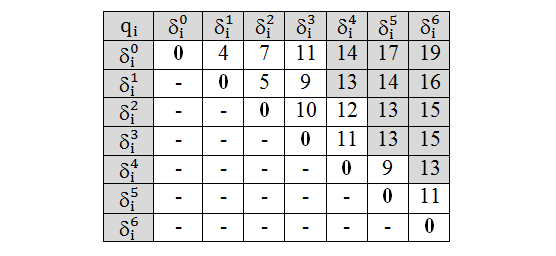
\includegraphics[width=0.45\textwidth]{algo_example_2.png}
\caption{Combined WCET and CPRD Costs.}
\label{fig:algo_example_2}
\end{center}
\vspace{-10pt}
\end{figure}
\begin{figure}[h!]
\vspace{-10pt}
\begin{center}
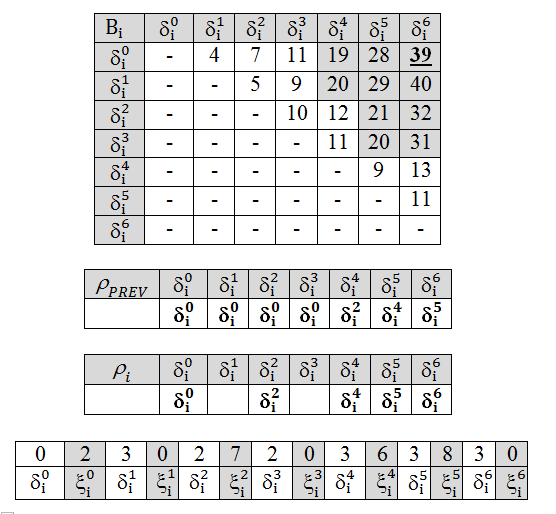
\includegraphics[width=0.45\textwidth]{algo_example_3.png}
\caption{Algorithm Results.}
\label{fig:algo_example_3}
\end{center}
\vspace{-10pt}
\end{figure}

\section{Evaluation}\label{sec:evaluation}

The evaluation of our preemption point placement algorithm will embody
two methods: 1) characterization and measurement of preemption costs
using real-time application code, and 2) a schedulability comparison
of synthetic task set for various preemption models. 

\subsection {Preemption Cost
  Characterization}\label{sec:preemption_cost_measurement} 
To characterize the behavior and estimate the benefit of the approach
proposed in this paper, a case study of representative tasks was
performed. The tasks were selected from Malardalen University of
Sweden's WCET benchmark suite \cite{mrtc:01}. Each task was built using Gaisler's
Bare-C Cross Compiler \cite{gaisler:01} for the GRSIM
LEON3 \cite{gaisler:02} simulated target. 

After compiling and linking, each task was analyzed by AbsInt's
a\textsuperscript{3} WCET \cite{absint:01} tool. This yielded the basic block
boundaries within each task. Next, the basic blocks
${\{B_1, B_2, ..., B_n\}}$ were serialized based upon an understanding of
the control flow of the task. Program points
${\{P_1, P_2, ..., P_n\}}$ were assigned by setting ${P_i}$ to the
address of the final instruction of each basic block ${B_i}$ for ${i}$
from ${0}$ to ${n}$.

Each program point ${P_j}$ served as a breakpoint within the task when
running on the simulator. The task was executed, recording the state of
the instruction ${C^I_j}$ and data ${C^D_j}$ cache state for every
visit of ${P_j}$. Given the limitations of the simulator and
a\textsuperscript{3} it was not possible record the actual control
flow. Thus, definitively over-estimating the UCBs shared between two
program points was not possible.

Instead, all instruction and data cache state was disregarded except
the state collected during the final visit of ${P_j}$ during the tasks
execution. Using these final snapshots the UCBs shared between two
program points ${P_i}$ and ${P_j}$ are determined by the following
equation. 
\begin{center}
  \begin{equation*}
    UCB(P_i, P_j) = \bigcap_{k=i}^{j-1} C_k
  \end{equation*}
\end{center}

In the equation above ${C}$ may be either the set of instruction or
data caches. This intersection of the cache state taken from program
point ${P_i}$ to the penultimate point ${P_{j-1}}$ serves as an upper
bound on the actual UCBs shared between the two points ${P_i}$ and
${P_j}$. Since the UCBs are the primary factor of CRPD, the results
are presented in terms of UCB counts.

\subsubsection{Availability}

This method may be verified and reproduced using the same tools and
data. Gaisler's compiler and simulator are freely available. AbsInt's
a\textsuperscript{3} tool is available for educational and evaluation
purposes. The programs written and data used in this paper can be
found on GitHub at the following url:

\begin{center}
https://github.com/ctessler/superblocks/tree/master/study
\end{center}


\subsubsection{Results}

The results are presented as a comparison between the method described
herein and the Bertonga approach. For a program point ${P_j}$ the
Bertogna approach defines the UCBs (and therefor the CRPD) as:

\begin{equation*}
  max\{ UCB(P_i, P_j) \vert i < j \}
\end{equation*}

To determine the maximum benefit of the new approach, the best case
scenario is considered. When the preemption point is selected with the
fewest number of UCBs based upon previous preemption.  For ${P_j}$ the
determination is made by:

\begin{equation*}
  min\{ UCB(P_i, P_j) \vert i < j \}
\end{equation*}


In the following graphs, each point in the graph represents two points
in the program. The first point of the program ${P_i}$ is fixed by the
x-axis. Each point in the graph is labelled with a number, a later
program point ${P_j}$ which has been selected by the the Bertogna
approach, or by the proposed method. Bertogna's approach follows the
dashed blue line, the proposed approach the solid black line.

Bertogna's approach is represented by the dashed blue line. The proposed
approach by the solid black line. Both approaches will select two
program points, represented by a single position in the
graph. Bertogna's approach would select the lowest value of the dashed
blue line. The proposed approach would select the lowest value of the
solid black line. Comparing the number of shared UCBs allows a
comparison to be made.

\begin{center}
  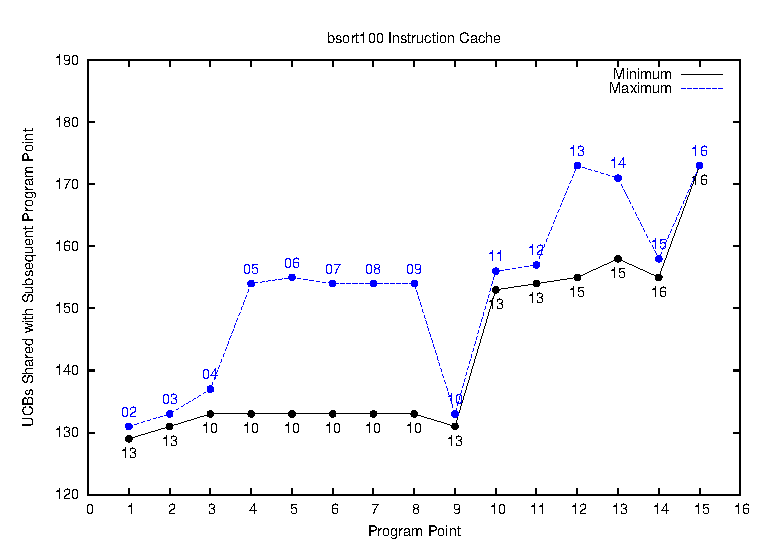
\includegraphics[width=\linewidth]{eps/bsort-icache.eps}
\end{center}

\begin{center}
  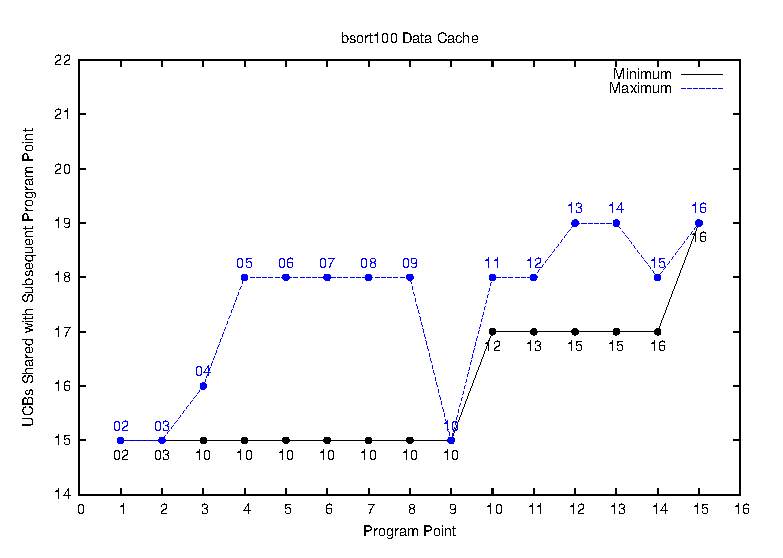
\includegraphics[width=\linewidth]{eps/bsort-dcache.eps}
\end{center}

\begin{center}
  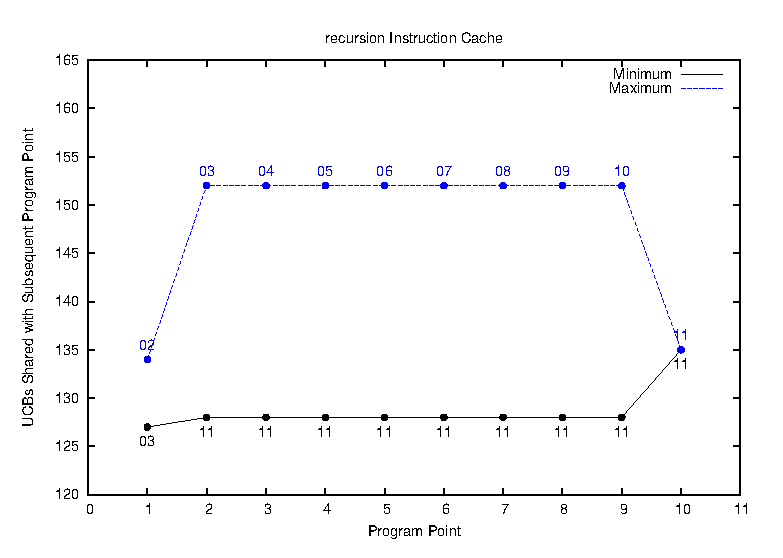
\includegraphics[width=\linewidth]{eps/recursion-icache.eps}
\end{center}

\begin{center}
  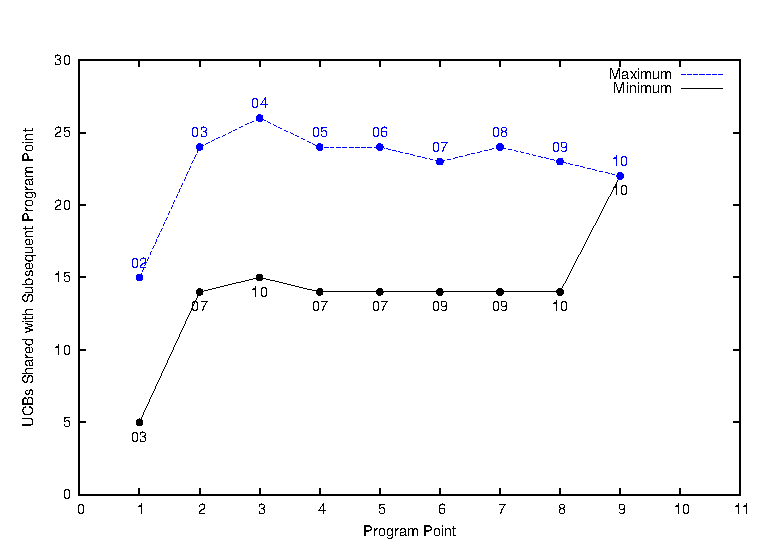
\includegraphics[width=\linewidth]{eps/recursion-dcache.eps}
\end{center}

%% An alternative for a wider graph
%% 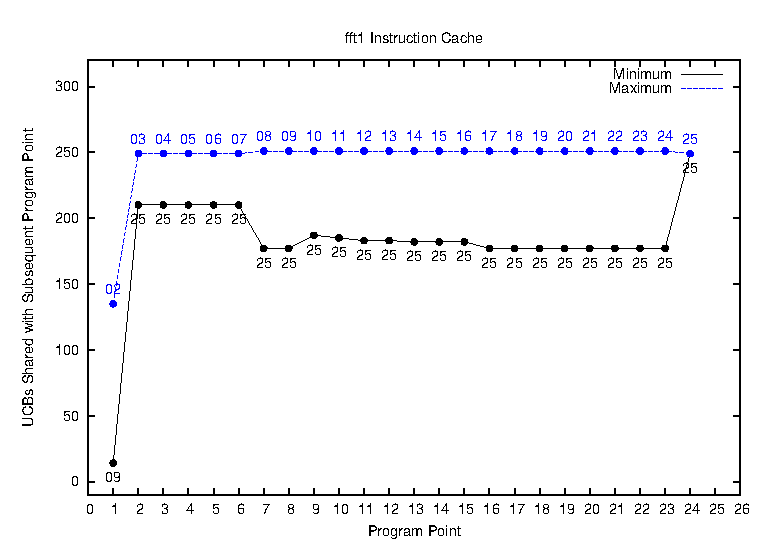
\includegraphics[width=\linewidth]{eps/fft1-icache.eps}

\begin{center}
  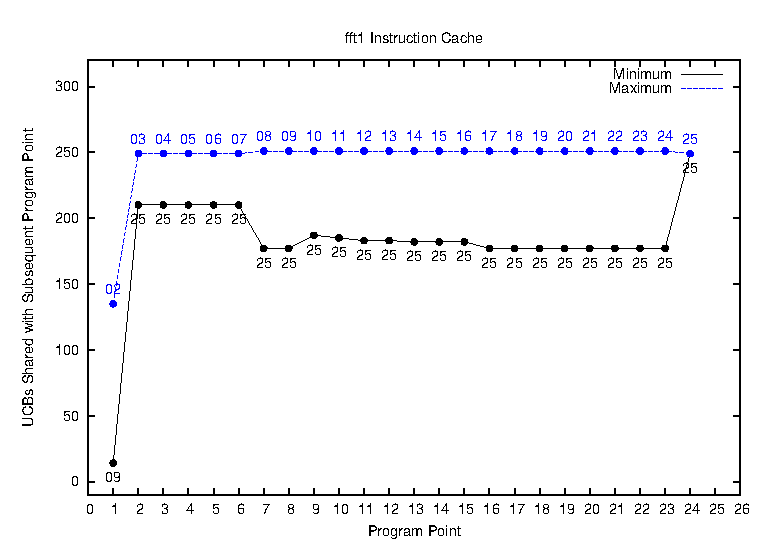
\includegraphics[width=\linewidth]{eps/fft1-icache.eps}
\end{center}

\begin{center}
  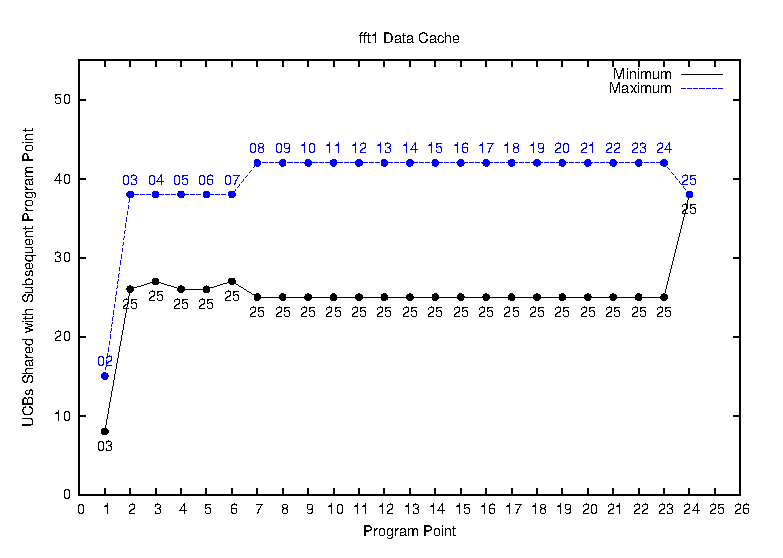
\includegraphics[width=\linewidth]{eps/fft1-dcache.eps}
\end{center}

For the bsort task, the proposed approach provides a benefit for the
instruction and data caches of 2 and 0 UCBs. For the fft1 task, the
instruction and data cache benefit is 121 and 7 UCBs. For the
recursion task, the benefit is 7 and 10 UCBs.


\subsection {Taskset Schedulability Evaluation}\label{sec:taskset schedulability}
The schedulability performance metrics we intend to compare various
preemption models with are: 1) the percentage of schedulable task sets
as a function of the task set utilization, 2) the percentage of
schedulable task sets as a function of the number of tasks, 3) the
percentage of schedulable task sets as a function of the maximum CRPD,
and 4) the percentage of schedulable task sets as a function of the
variability of the CRPD variance \begin{math}\sigma_{CRPD}\end{math}.
The following preemption models will be studied namely: 1) fully
non-preemptive, 2) fully preemptive, 3) limited preemption naive
approach, 4) limited preemption point placement with fixed CRPD
preemption cost, 5) limited preemption point placement with variable
CRPD preemption cost, and 6) optimal preemption point placement with
enhanced CRPD preemption cost. 

Our approach for generating the synthetic task sets involves a number
of steps which is summarized as follows.  The number of basic blocks
generated each task is in the
interval \begin{math}[N_{i}(min),N_{i}(max)]\end{math} using a random
uniform distribution.  Each basic block non-preemptive WCET is
generated using a Gaussian distribution with
mean \begin{math}\mu_{WCET}\end{math} and
variance \begin{math}\sigma_{WCET}\end{math}.  The  utilization of
each task has been generated using the approach proposed in [TBD12].
The task periods \begin{math}T_{i}\end{math} were then computed
dividing the non-preemptive WCET \begin{math}C_{i}^{NP}\end{math} by
the utilization \begin{math}U_{i}\end{math} of each task.  Preemption
costs were randomly generated using the following function (TBD), to
achieve a realistic distribution similar to the one derived
empirically).  The enhanced CRPD is generated to be a percentage of
the WCET in the interval [0, 0.50] with a random uniform
distribution. Cache related preemption delay (CRPD) values are
generated for each pair of potential preemption points.  The variable
CRPD preemption cost model uses the CRPD cost from the each preemption
point to the end of the task. The fixed CRPD preemption cost model
uses the maximum CRPD cost of all variable CRPD preemption cost
values.  

\section{Conclusion}\label{sec:conclusion}

In this paper we presented an enhanced approach for calculating the
CRPD taking into account the selected preemption points resulting
in greater accuracy.  Using a more precise CRPD calculation, we also
presented an improved algorithm for selecting a limited number of
preemption points for each task subject to schedulability constraints.
Our improved preemption placement algorithm was demonstrated to
minimize the overall preemption cost, an important result in achieving
schedulability in real-time systems.  We highlighted the iterative nature
of considering schedulability constraints in our preemption point
placement algorithm and proposed an algorithm combining schedulability
analysis with limited preemption point placement.  This approach
effectively illustrates how the individual tasks non-preemption
region parameters $Q_i$ and the optimal selected preemption points will
eventually converge.  Furthermore, our enhanced algorithm was demonstrated to be
optimal in that if a feasible schedule is not found, then no feasible
schedule exists by any known method utilizing a static $Q_i$ value.  Our algorithm
was shown to run in quadratic time complexity.  Potential preemption points can be
defined automatically using Gaisler's compiler and simulator along with AbsInt's
a\textsuperscript{3} tool or defined manually by the programmer during design
and implementation. Our experiments demonstrated the effectiveness of
the enhanced CRPD calculation by illustrating the benefits using the
task set from the MRTC WCET benchmark suite~\cite{mrtc:01}.
We also demonstrated the benefits of our enhanced limited optimal preemption
point placement algorithm and its increased system schedulability as
compared to other algorithms.  While our task model is defined using a linear
sequence of basic blocks, it was deemed a highly suitable model to introduce
our revised methods for enhanced CRPD calculation and optimal limited
preemption point placement.  The need to subsume higher level programming constructs
being the prominent assumption of the linear basic block structure can potentially
diminish the utility of our approach if the non-preemptive execution time of any basic block
violates the constraint \begin{math}C_{i}^{NP}\end{math} \begin{math}>\end{math} \begin{math}Q_{i}\end{math}.  For this case, we need to ``break-up'' the basic block by permitting preemption every $Q_i$ time units.
%To overcome this limitation in future work, we plan to relax the linear basic block structure assumption and
%address arbitrarily connected basic block structures.

In future work, we plan to 1) extend the techniques described here to set-associative caches,
2) perform a schedulability comparison of synthetic task set for various preemption models, and
3) remove the linear basic block restriction thereby permitting arbitrary control flowgraphs.

%%
\clearpage
%
\section{Appendix}\label{sec:appendix}
%
\vspace{-20pt}
\begin{figure}[h!]
\begin{center}
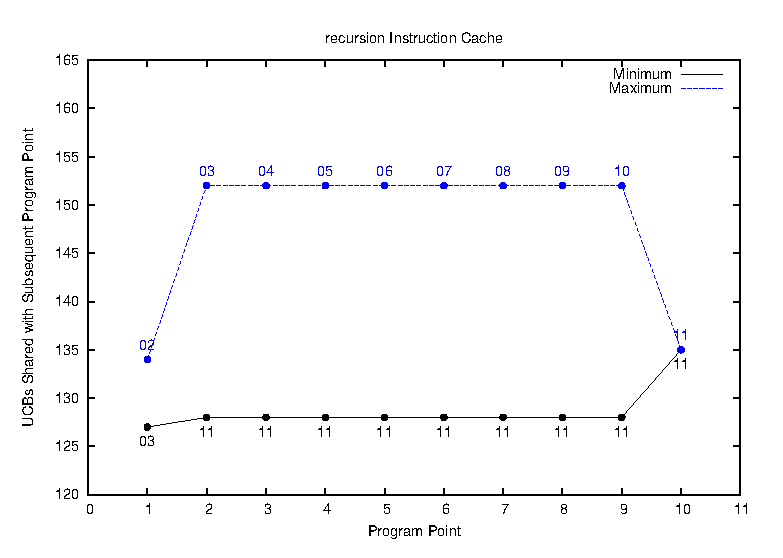
\includegraphics[width=\linewidth]{eps/recursion-icache.eps}
\caption{Recursion Instruction Cache.}
\label{fig:recursion_instruction_cache}
\end{center}
\end{figure}
%
\vspace{-20pt}
\begin{figure}[h!]
\begin{center}
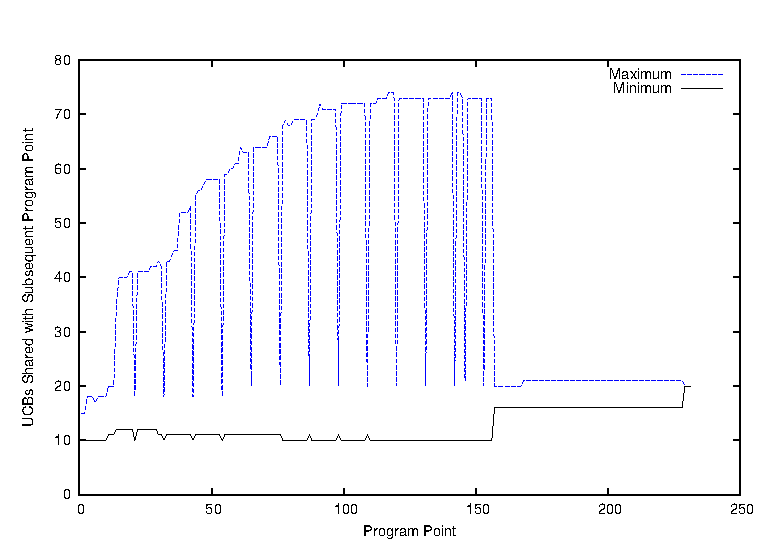
\includegraphics[width=\linewidth]{eps/adpcm-dcache.eps}
\caption{ADPCM Data Cache.}
\label{fig:adpcm_data_cache}
\end{center}
\end{figure}
%
\vspace{-20pt}
\begin{figure}[h!]
\begin{center}
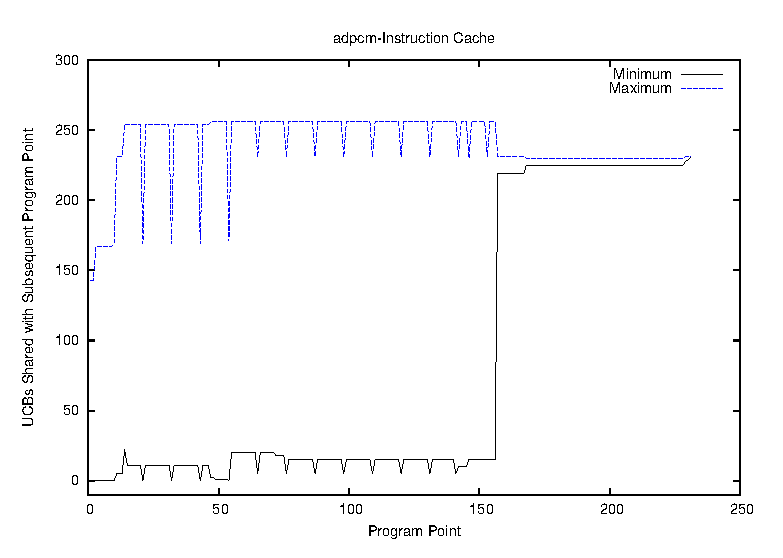
\includegraphics[width=\linewidth]{eps/adpcm-icache.eps}
\caption{ADPCM Instruction Cache.}
\label{fig:adpcm_instruction_cache}
\end{center}
\end{figure}
%
\vspace{-20pt}
\begin{figure}[h!]
\begin{center}
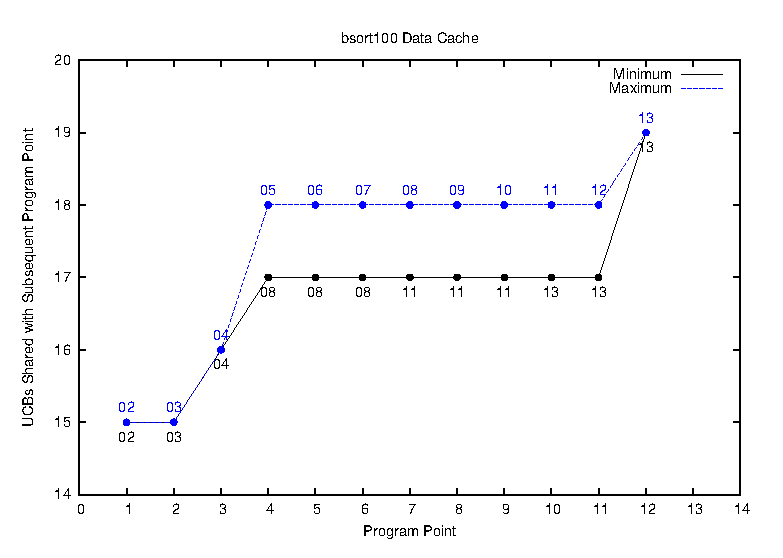
\includegraphics[width=\linewidth]{eps/bsort100-dcache.eps}
\caption{BSORT100 Data Cache.}
\label{fig:bsort100_data_cache}
\end{center}
\end{figure}
%
\vspace{-20pt}
\begin{figure}[h!]
\begin{center}
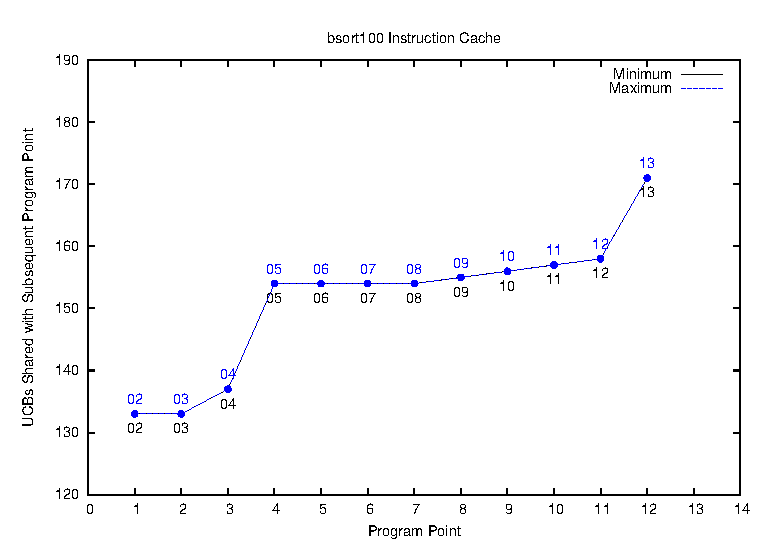
\includegraphics[width=\linewidth]{eps/bsort100-icache.eps}
\caption{BSORT100 Instruction Cache.}
\label{fig:bsort100_instruction_cache}
\end{center}
\end{figure}
%
\vspace{-20pt}
\begin{figure}[h!]
\begin{center}
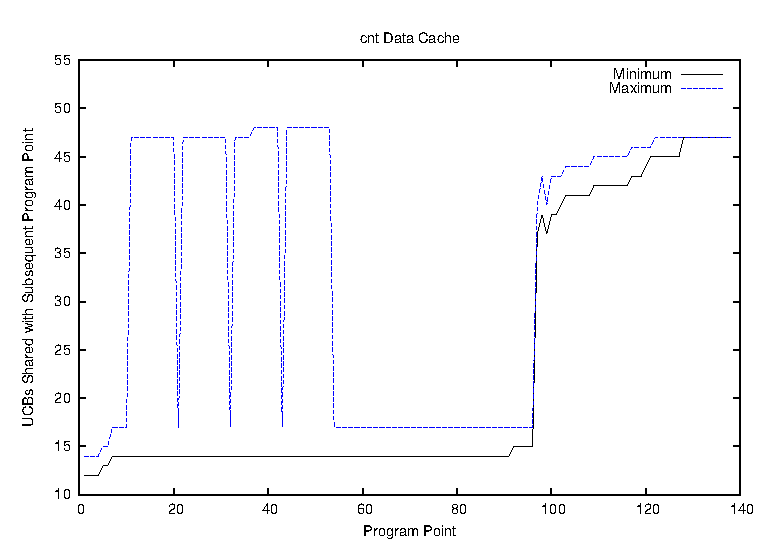
\includegraphics[width=\linewidth]{eps/cnt-dcache.eps}
\caption{CNT Data Cache.}
\label{fig:cnt_data_cache}
\end{center}
\end{figure}
%
\vspace{-20pt}
\begin{figure}[h!]
\begin{center}
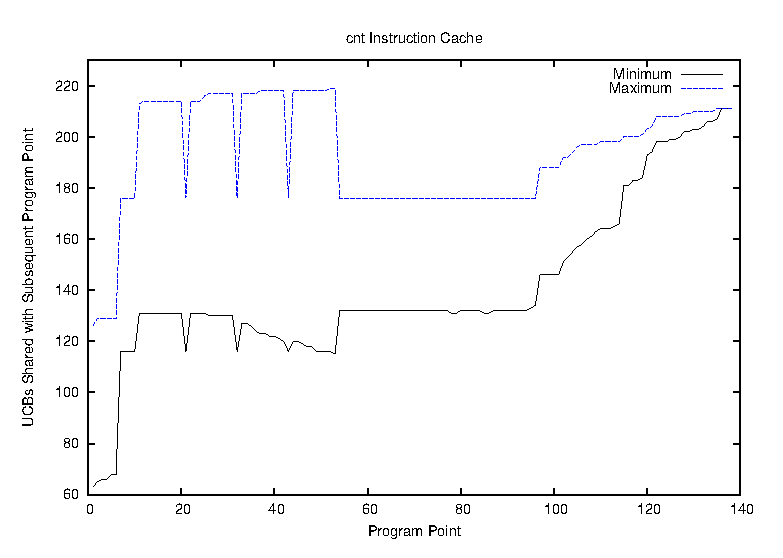
\includegraphics[width=\linewidth]{eps/cnt-icache.eps}
\caption{CNT Instruction Cache.}
\label{fig:cnt_instruction_cache}
\end{center}
\end{figure}
%
\vspace{-20pt}
\begin{figure}[h!]
\begin{center}
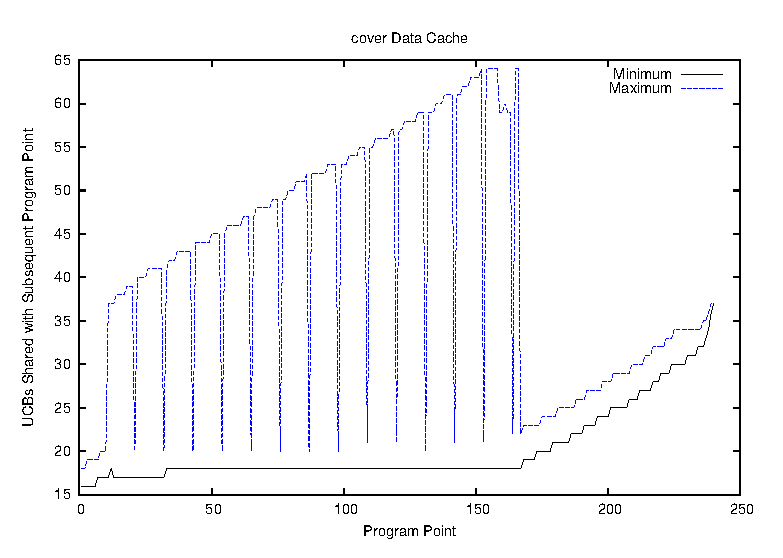
\includegraphics[width=\linewidth]{eps/cover-dcache.eps}
\caption{Cover Data Cache.}
\label{fig:cover_data_cache}
\end{center}
\end{figure}
%
\vspace{-20pt}
\begin{figure}[h!]
\begin{center}
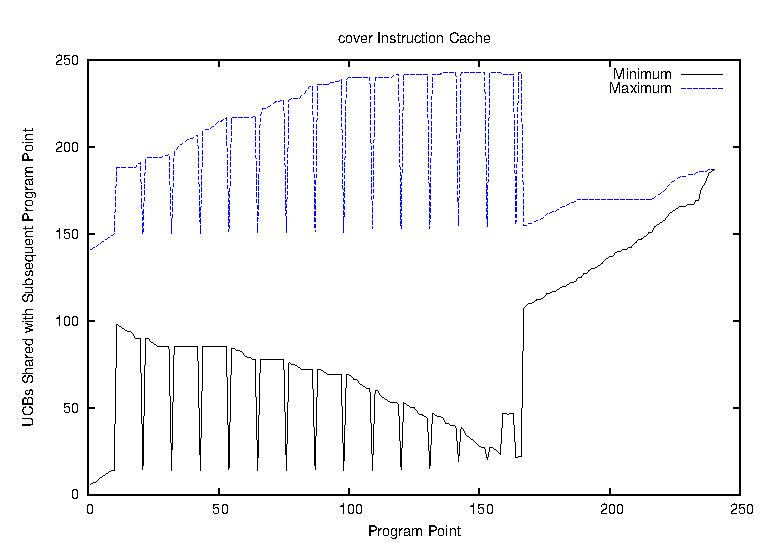
\includegraphics[width=\linewidth]{eps/cover-icache.eps}
\caption{Cover Instruction Cache.}
\label{fig:cover_instruction_cache}
\end{center}
\end{figure}
%
\vspace{-20pt}
\begin{figure}[h!]
\begin{center}
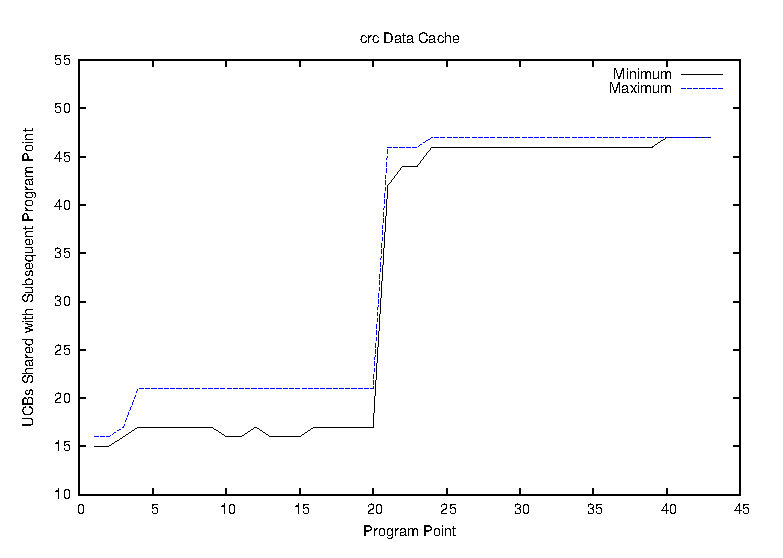
\includegraphics[width=\linewidth]{eps/crc-dcache.eps}
\caption{CRC Data Cache.}
\label{fig:crc_data_cache}
\end{center}
\end{figure}
%
\vspace{-20pt}
\begin{figure}[h!]
\begin{center}
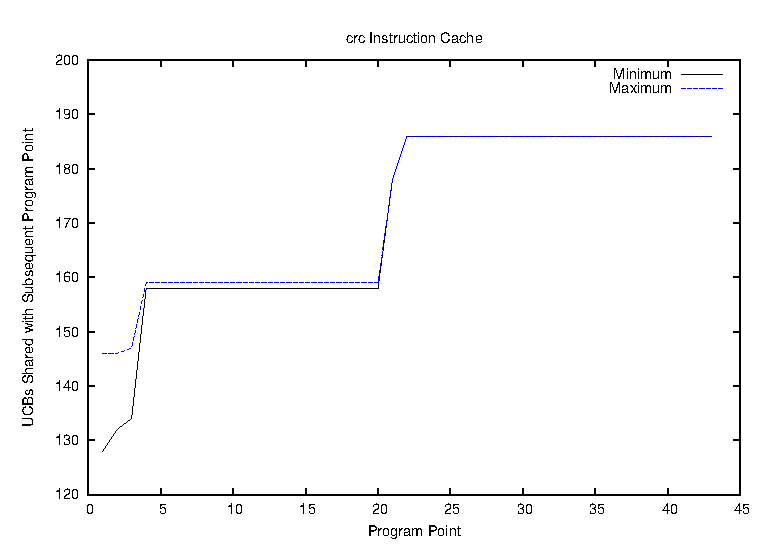
\includegraphics[width=\linewidth]{eps/crc-icache.eps}
\caption{CRC Instruction Cache.}
\label{fig:crc_instruction_cache}
\end{center}
\end{figure}
%
\vspace{-20pt}
\begin{figure}[h!]
\begin{center}
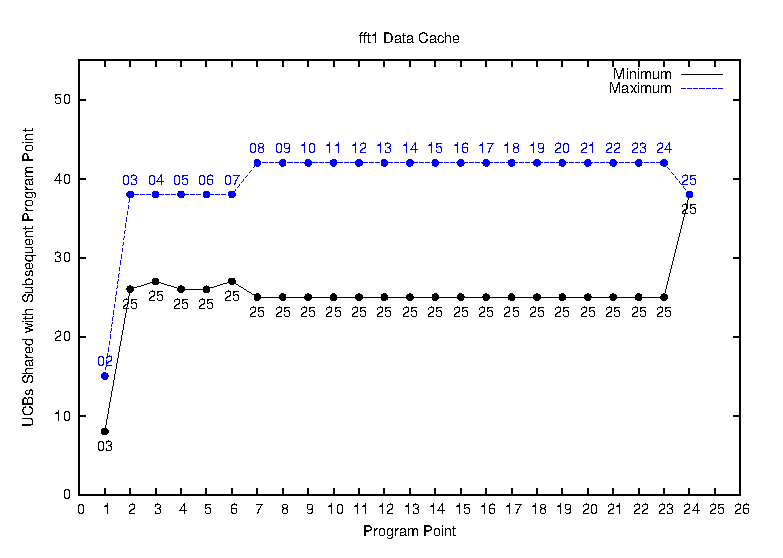
\includegraphics[width=\linewidth]{eps/fft1-dcache.eps}
\caption{FFT1 Data Cache.}
\label{fig:fft1_data_cache}
\end{center}
\end{figure}
%
\vspace{-20pt}
\begin{figure}[h!]
\begin{center}
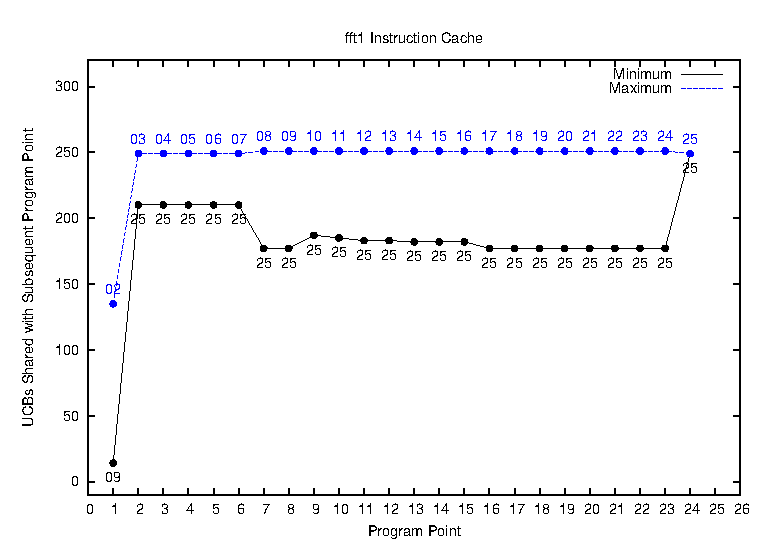
\includegraphics[width=\linewidth]{eps/fft1-icache.eps}
\caption{FFT1 Instruction Cache.}
\label{fig:fft1_instruction_cache}
\end{center}
\end{figure}
%
\vspace{-20pt}
\begin{figure}[h!]
\begin{center}
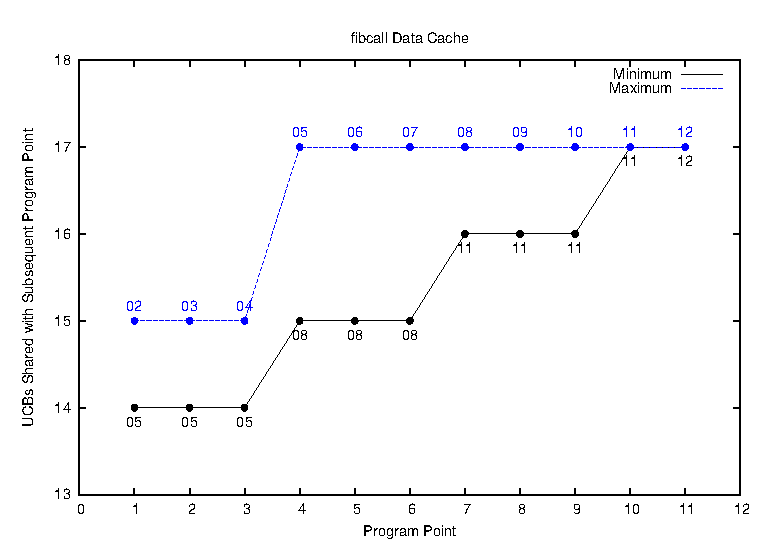
\includegraphics[width=\linewidth]{eps/fibcall-dcache.eps}
\caption{Fibcall Data Cache.}
\label{fig:fibcall_data_cache}
\end{center}
\end{figure}
%
\vspace{-20pt}
\begin{figure}[h!]
\begin{center}
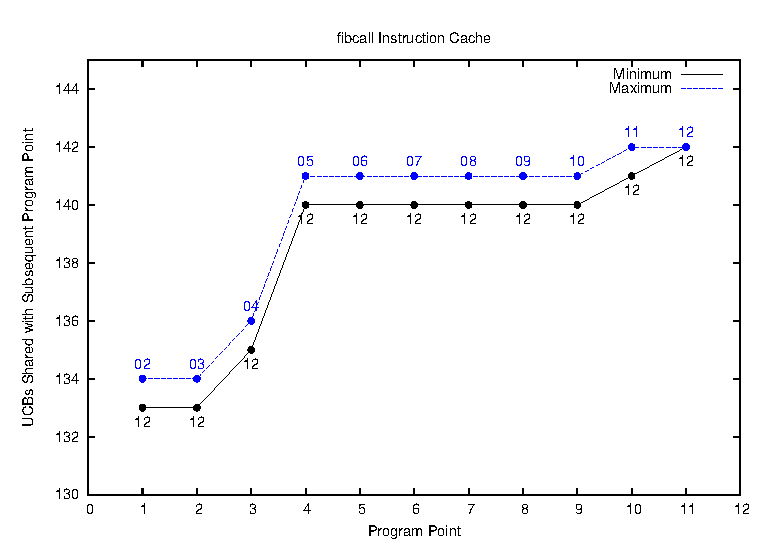
\includegraphics[width=\linewidth]{eps/fibcall-icache.eps}
\caption{Fibcall Instruction Cache.}
\label{fig:fibcall_instruction_cache}
\end{center}
\end{figure}
%
\begin{figure}[h!]
\vspace{-20pt}
\begin{center}
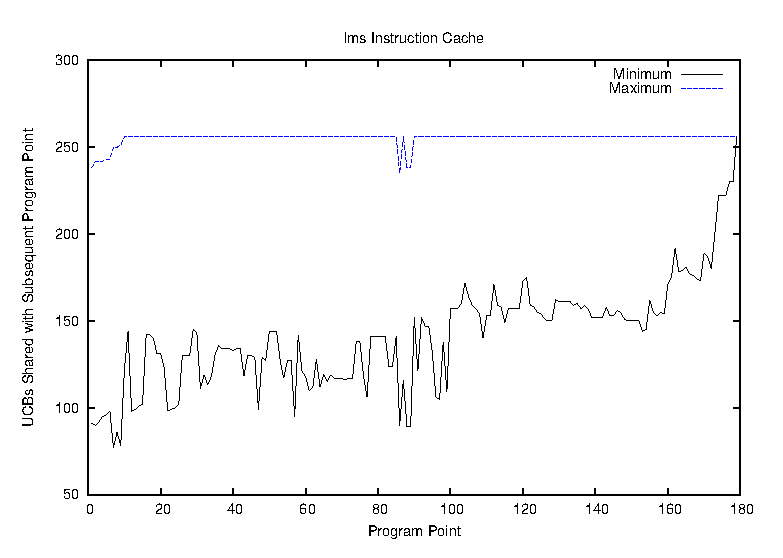
\includegraphics[width=\linewidth]{eps/lms-icache.eps}
\caption{LMS Instruction Cache.}
\label{fig:lms_instruction_cache}
\end{center}
\vspace{-10pt}
\end{figure}
%
\vspace{-20pt}
\begin{figure}[h!]
\begin{center}
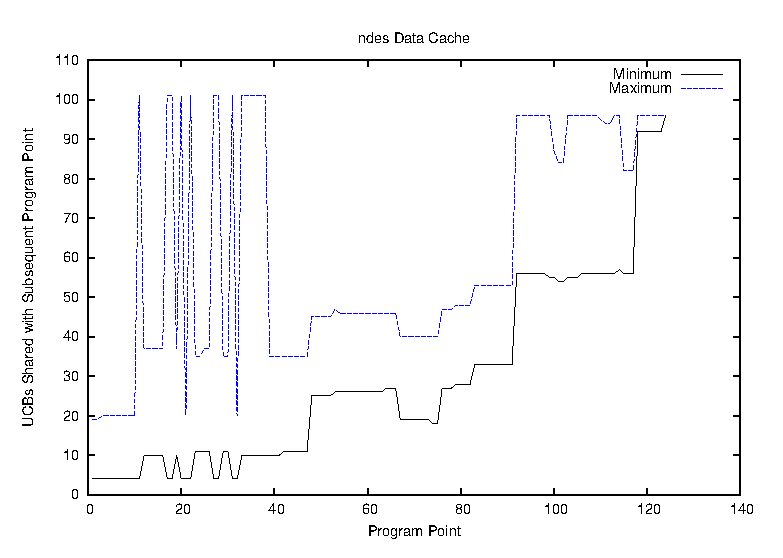
\includegraphics[width=\linewidth]{eps/ndes-dcache.eps}
\caption{NDES Data Cache.}
\label{fig:ndes_data_cache}
\end{center}
\end{figure}
%
\vspace{-20pt}
\begin{figure}[h!]
\begin{center}
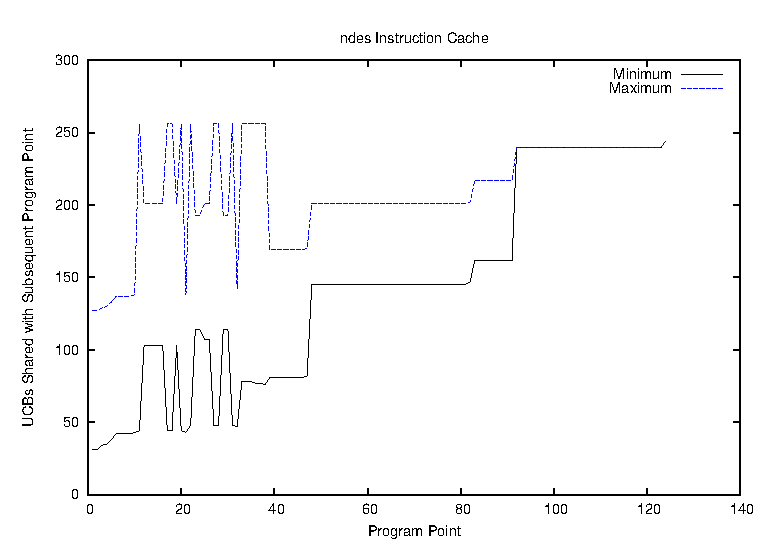
\includegraphics[width=\linewidth]{eps/ndes-icache.eps}
\caption{NDES Instruction Cache.}
\label{fig:ndes_instruction_cache}
\end{center}
\end{figure}
% 



\scriptsize\addtolength{\baselineskip}{-2mm}
\bibliographystyle{IEEEtran}
\bibliography{web-bib}

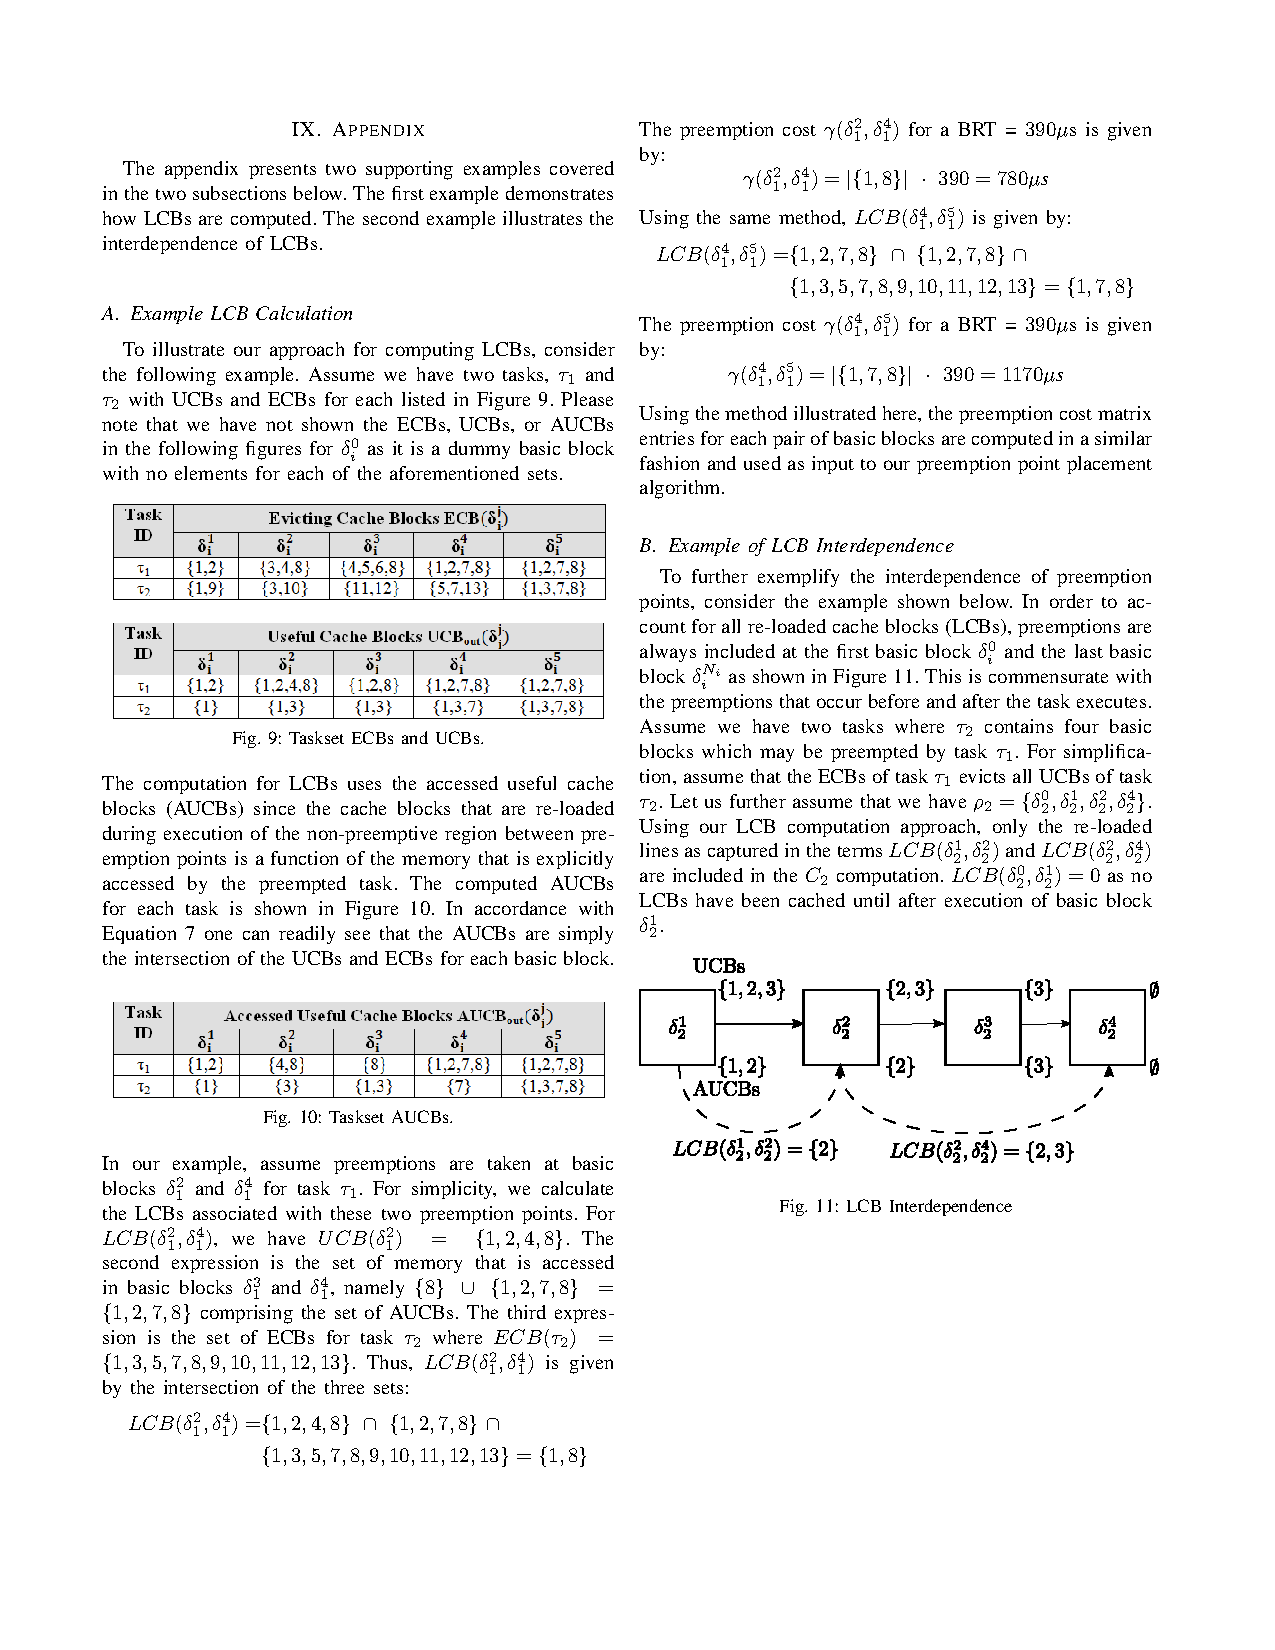
\includepdf[pages=1]{crpd_lppp_appendix}

%end document
\end{document}

